\documentclass[twoside]{book}

% Packages required by doxygen
\usepackage{fixltx2e}
\usepackage{calc}
\usepackage{doxygen}
\usepackage[export]{adjustbox} % also loads graphicx
\usepackage{graphicx}
\usepackage[utf8]{inputenc}
\usepackage{makeidx}
\usepackage{multicol}
\usepackage{multirow}
\PassOptionsToPackage{warn}{textcomp}
\usepackage{textcomp}
\usepackage[nointegrals]{wasysym}
\usepackage[table]{xcolor}

% Font selection
\usepackage[T1]{fontenc}
\usepackage[scaled=.90]{helvet}
\usepackage{courier}
\usepackage{amssymb}
\usepackage{sectsty}
\renewcommand{\familydefault}{\sfdefault}
\allsectionsfont{%
  \fontseries{bc}\selectfont%
  \color{darkgray}%
}
\renewcommand{\DoxyLabelFont}{%
  \fontseries{bc}\selectfont%
  \color{darkgray}%
}
\newcommand{\+}{\discretionary{\mbox{\scriptsize$\hookleftarrow$}}{}{}}

% Page & text layout
\usepackage{geometry}
\geometry{%
  a4paper,%
  top=2.5cm,%
  bottom=2.5cm,%
  left=2.5cm,%
  right=2.5cm%
}
\tolerance=750
\hfuzz=15pt
\hbadness=750
\setlength{\emergencystretch}{15pt}
\setlength{\parindent}{0cm}
\setlength{\parskip}{3ex plus 2ex minus 2ex}
\makeatletter
\renewcommand{\paragraph}{%
  \@startsection{paragraph}{4}{0ex}{-1.0ex}{1.0ex}{%
    \normalfont\normalsize\bfseries\SS@parafont%
  }%
}
\renewcommand{\subparagraph}{%
  \@startsection{subparagraph}{5}{0ex}{-1.0ex}{1.0ex}{%
    \normalfont\normalsize\bfseries\SS@subparafont%
  }%
}
\makeatother

% Headers & footers
\usepackage{fancyhdr}
\pagestyle{fancyplain}
\fancyhead[LE]{\fancyplain{}{\bfseries\thepage}}
\fancyhead[CE]{\fancyplain{}{}}
\fancyhead[RE]{\fancyplain{}{\bfseries\leftmark}}
\fancyhead[LO]{\fancyplain{}{\bfseries\rightmark}}
\fancyhead[CO]{\fancyplain{}{}}
\fancyhead[RO]{\fancyplain{}{\bfseries\thepage}}
\fancyfoot[LE]{\fancyplain{}{}}
\fancyfoot[CE]{\fancyplain{}{}}
\fancyfoot[RE]{\fancyplain{}{\bfseries\scriptsize Generated by Doxygen }}
\fancyfoot[LO]{\fancyplain{}{\bfseries\scriptsize Generated by Doxygen }}
\fancyfoot[CO]{\fancyplain{}{}}
\fancyfoot[RO]{\fancyplain{}{}}
\renewcommand{\footrulewidth}{0.4pt}
\renewcommand{\chaptermark}[1]{%
  \markboth{#1}{}%
}
\renewcommand{\sectionmark}[1]{%
  \markright{\thesection\ #1}%
}

% Indices & bibliography
\usepackage{natbib}
\usepackage[titles]{tocloft}
\setcounter{tocdepth}{3}
\setcounter{secnumdepth}{5}
\makeindex

% Hyperlinks (required, but should be loaded last)
\usepackage{ifpdf}
\ifpdf
  \usepackage[pdftex,pagebackref=true]{hyperref}
\else
  \usepackage[ps2pdf,pagebackref=true]{hyperref}
\fi
\hypersetup{%
  colorlinks=true,%
  linkcolor=blue,%
  citecolor=blue,%
  unicode%
}

% Custom commands
\newcommand{\clearemptydoublepage}{%
  \newpage{\pagestyle{empty}\cleardoublepage}%
}

\usepackage{caption}
\captionsetup{labelsep=space,justification=centering,font={bf},singlelinecheck=off,skip=4pt,position=top}

%===== C O N T E N T S =====

\begin{document}

% Titlepage & ToC
\hypersetup{pageanchor=false,
             bookmarksnumbered=true,
             pdfencoding=unicode
            }
\pagenumbering{alph}
\begin{titlepage}
\vspace*{7cm}
\begin{center}%
{\Large My Project }\\
\vspace*{1cm}
{\large Generated by Doxygen 1.8.13}\\
\end{center}
\end{titlepage}
\clearemptydoublepage
\pagenumbering{roman}
\tableofcontents
\clearemptydoublepage
\pagenumbering{arabic}
\hypersetup{pageanchor=true}

%--- Begin generated contents ---
\chapter{M\+I\+A\+\_\+\+P\+Y1\+\_\+\+F\+A\+S\+E1}
\label{md_README}
\Hypertarget{md_README}
Fase 1 del proyecto 1 de Manejo e implementación de archivos, implementación de una aplicación de consola siguiendo patrones de diseño Interpreter, se implementa un sistema R\+A\+ID en conjunto con un simulador de E\+X\+T3. 
\chapter{Class Index}
\section{Class List}
Here are the classes, structs, unions and interfaces with brief descriptions\+:\begin{DoxyCompactList}
\item\contentsline{section}{\hyperlink{structEBR}{E\+BR} }{\pageref{structEBR}}{}
\item\contentsline{section}{\hyperlink{classFDISK__}{F\+D\+I\+S\+K\+\_\+} \\*Clase en la que se programaron el análisis semantico de la función F\+D\+I\+SK además se implemento su funcionamiento y validación de parámetros }{\pageref{classFDISK__}}{}
\item\contentsline{section}{\hyperlink{structMBR}{M\+BR} }{\pageref{structMBR}}{}
\item\contentsline{section}{\hyperlink{classMKDISK__}{M\+K\+D\+I\+S\+K\+\_\+} }{\pageref{classMKDISK__}}{}
\item\contentsline{section}{\hyperlink{classMOUNT__}{M\+O\+U\+N\+T\+\_\+} }{\pageref{classMOUNT__}}{}
\item\contentsline{section}{\hyperlink{structPartition}{Partition} }{\pageref{structPartition}}{}
\item\contentsline{section}{\hyperlink{classREP__}{R\+E\+P\+\_\+} }{\pageref{classREP__}}{}
\item\contentsline{section}{\hyperlink{classRMDISK__}{R\+M\+D\+I\+S\+K\+\_\+} }{\pageref{classRMDISK__}}{}
\item\contentsline{section}{\hyperlink{classUNMOUNT__}{U\+N\+M\+O\+U\+N\+T\+\_\+} }{\pageref{classUNMOUNT__}}{}
\item\contentsline{section}{\hyperlink{structyy__buffer__state}{yy\+\_\+buffer\+\_\+state} }{\pageref{structyy__buffer__state}}{}
\item\contentsline{section}{\hyperlink{structyy__trans__info}{yy\+\_\+trans\+\_\+info} }{\pageref{structyy__trans__info}}{}
\item\contentsline{section}{\hyperlink{unionyyalloc}{yyalloc} }{\pageref{unionyyalloc}}{}
\item\contentsline{section}{\hyperlink{structYYLTYPE}{Y\+Y\+L\+T\+Y\+PE} }{\pageref{structYYLTYPE}}{}
\item\contentsline{section}{\hyperlink{unionYYSTYPE}{Y\+Y\+S\+T\+Y\+PE} }{\pageref{unionYYSTYPE}}{}
\end{DoxyCompactList}

\chapter{Class Documentation}
\hypertarget{structEBR}{}\section{E\+BR Struct Reference}
\label{structEBR}\index{E\+BR@{E\+BR}}


{\ttfamily \#include $<$structs.\+h$>$}

\subsection*{Public Attributes}
\begin{DoxyCompactItemize}
\item 
\mbox{\Hypertarget{structEBR_a4ce8f52d4855da2b30a15ed463266e82}\label{structEBR_a4ce8f52d4855da2b30a15ed463266e82}} 
char {\bfseries part\+\_\+status} =\textquotesingle{}0\textquotesingle{}
\item 
\mbox{\Hypertarget{structEBR_a291d77cd42d2bed928d43861f1fad4aa}\label{structEBR_a291d77cd42d2bed928d43861f1fad4aa}} 
char {\bfseries part\+\_\+fit} =\textquotesingle{}0\textquotesingle{}
\item 
\mbox{\Hypertarget{structEBR_a66db820ea0adcca22c76c136e2fabfbe}\label{structEBR_a66db820ea0adcca22c76c136e2fabfbe}} 
int {\bfseries part\+\_\+start} =-\/1
\item 
\mbox{\Hypertarget{structEBR_a4ff5eb013c47054ac5bb1a1d79389d47}\label{structEBR_a4ff5eb013c47054ac5bb1a1d79389d47}} 
int {\bfseries part\+\_\+size} =0
\item 
\mbox{\Hypertarget{structEBR_a6d2159ec6ead1ac0384b99902180c72b}\label{structEBR_a6d2159ec6ead1ac0384b99902180c72b}} 
int {\bfseries part\+\_\+next} =-\/1
\item 
\mbox{\Hypertarget{structEBR_a365cfcb47bff391be6a06fb65fd1da4f}\label{structEBR_a365cfcb47bff391be6a06fb65fd1da4f}} 
char {\bfseries part\+\_\+name} \mbox{[}16\mbox{]}
\end{DoxyCompactItemize}


\subsection{Detailed Description}
Particiones lógicas. 

The documentation for this struct was generated from the following file\+:\begin{DoxyCompactItemize}
\item 
structs.\+h\end{DoxyCompactItemize}

\hypertarget{classFDISK__}{}\section{F\+D\+I\+S\+K\+\_\+ Class Reference}
\label{classFDISK__}\index{F\+D\+I\+S\+K\+\_\+@{F\+D\+I\+S\+K\+\_\+}}


Clase en la que se programaron el análisis semantico de la función F\+D\+I\+SK además se implemento su funcionamiento y validación de parámetros.  




{\ttfamily \#include $<$F\+D\+I\+S\+K.\+h$>$}

\subsection*{Public Member Functions}
\begin{DoxyCompactItemize}
\item 
\hyperlink{classFDISK___a418b57a089062accc33338bcbb9daec4}{F\+D\+I\+S\+K\+\_\+} ()
\item 
void \hyperlink{classFDISK___ac62891d61885c9e3e5d416b11f067c5b}{set\+Size} (char $\ast$size)
\item 
void \hyperlink{classFDISK___ac829852f41210c96957753e611c96c32}{set\+Unit} (char $\ast$unit)
\item 
void \hyperlink{classFDISK___a7dbf2da61853e0ac59c6ce48862d4013}{set\+Path} (char $\ast$path)
\item 
void \hyperlink{classFDISK___afb2ab7c0bdd1584aa5cb977de810bdd4}{set\+Fit} (char $\ast$fit)
\item 
void \hyperlink{classFDISK___ae5113216c8167ca54b1d5a99d29ed963}{set\+Delete} (char $\ast$\+\_\+delete)
\item 
void \hyperlink{classFDISK___a28bccf6dd576824e040a29b389c8a650}{set\+Name} (char $\ast$name)
\item 
void \hyperlink{classFDISK___a6de35bf474b492d03494d5cdf373df1a}{set\+Add} (char $\ast$add)
\item 
void \hyperlink{classFDISK___a95fb02a0658219e583601de4844a517c}{set\+Correct} (bool correct)
\item 
void \hyperlink{classFDISK___aa45b16384c955ecb2c7f0a02f8e62bb0}{set\+Type} (char $\ast$type)
\item 
char \hyperlink{classFDISK___af29e537ad425951e4c4379f812d18a21}{get\+Fit} ()
\item 
char \hyperlink{classFDISK___abb61ba4d1545287d53bca288bc3ae244}{get\+Unit} ()
\item 
int \hyperlink{classFDISK___a36811336ad11d30c712b2a9760286087}{get\+Size} ()
\item 
signed char \hyperlink{classFDISK___a7e5bbf0438a218aabb09bea7dfb2f9ef}{get\+Type} ()
\item 
void \hyperlink{classFDISK___a1d030793b942f70d9cde1d7bd7a2bb36}{create\+Part} ()
\item 
void \hyperlink{classFDISK___a34427ce807ae61a1e0b101bb2a69b581}{primary\+Part} (kink which)
\item 
void \hyperlink{classFDISK___a03f9fa267b7bdf7b2dda3aa13cfc960d}{extended\+Part} (kink which)
\item 
void \hyperlink{classFDISK___aabd69e0175b1950638c51ccf26cb0dcb}{logic\+Part} (kink which)
\item 
bool \hyperlink{classFDISK___a93bf6bebd83704cc477d365c52e78cca}{does\+Exist} (char $\ast$name, kink which)
\item 
void \hyperlink{classFDISK___a48abd8fe6a02cabd370e02a2b87164a3}{print\+End} (kink which)
\item 
void \hyperlink{classFDISK___a926ec9e4cadf17773cc630e0423af3db}{modify\+Part} ()
\item 
void \hyperlink{classFDISK___ac066192fc5d768882f553a802e34a1fd}{delete\+Part} ()
\item 
void \hyperlink{classFDISK___a3cabb04c96798f42985d7c199ba1987f}{semantic} ()
\item 
void \hyperlink{classFDISK___a00c4753fc48745eaf7b9fab40e864a94}{run} ()
\item 
void \hyperlink{classFDISK___ac3a1b362131afe438a0cfcd55d24fb24}{Debug\+Binario} ()
\end{DoxyCompactItemize}


\subsection{Detailed Description}
Clase en la que se programaron el análisis semantico de la función F\+D\+I\+SK además se implemento su funcionamiento y validación de parámetros. 

\subsection{Constructor \& Destructor Documentation}
\mbox{\Hypertarget{classFDISK___a418b57a089062accc33338bcbb9daec4}\label{classFDISK___a418b57a089062accc33338bcbb9daec4}} 
\index{F\+D\+I\+S\+K\+\_\+@{F\+D\+I\+S\+K\+\_\+}!F\+D\+I\+S\+K\+\_\+@{F\+D\+I\+S\+K\+\_\+}}
\index{F\+D\+I\+S\+K\+\_\+@{F\+D\+I\+S\+K\+\_\+}!F\+D\+I\+S\+K\+\_\+@{F\+D\+I\+S\+K\+\_\+}}
\subsubsection{\texorpdfstring{F\+D\+I\+S\+K\+\_\+()}{FDISK\_()}}
{\footnotesize\ttfamily F\+D\+I\+S\+K\+\_\+\+::\+F\+D\+I\+S\+K\+\_\+ (\begin{DoxyParamCaption}{ }\end{DoxyParamCaption})\hspace{0.3cm}{\ttfamily [inline]}}

Constructor vacio del objeto 

\subsection{Member Function Documentation}
\mbox{\Hypertarget{classFDISK___a1d030793b942f70d9cde1d7bd7a2bb36}\label{classFDISK___a1d030793b942f70d9cde1d7bd7a2bb36}} 
\index{F\+D\+I\+S\+K\+\_\+@{F\+D\+I\+S\+K\+\_\+}!create\+Part@{create\+Part}}
\index{create\+Part@{create\+Part}!F\+D\+I\+S\+K\+\_\+@{F\+D\+I\+S\+K\+\_\+}}
\subsubsection{\texorpdfstring{create\+Part()}{createPart()}}
{\footnotesize\ttfamily void F\+D\+I\+S\+K\+\_\+\+::create\+Part (\begin{DoxyParamCaption}{ }\end{DoxyParamCaption})\hspace{0.3cm}{\ttfamily [inline]}}

Metodo para crear particion \mbox{\Hypertarget{classFDISK___ac3a1b362131afe438a0cfcd55d24fb24}\label{classFDISK___ac3a1b362131afe438a0cfcd55d24fb24}} 
\index{F\+D\+I\+S\+K\+\_\+@{F\+D\+I\+S\+K\+\_\+}!Debug\+Binario@{Debug\+Binario}}
\index{Debug\+Binario@{Debug\+Binario}!F\+D\+I\+S\+K\+\_\+@{F\+D\+I\+S\+K\+\_\+}}
\subsubsection{\texorpdfstring{Debug\+Binario()}{DebugBinario()}}
{\footnotesize\ttfamily void F\+D\+I\+S\+K\+\_\+\+::\+Debug\+Binario (\begin{DoxyParamCaption}{ }\end{DoxyParamCaption})\hspace{0.3cm}{\ttfamily [inline]}}

Método para imprimir el \hyperlink{structMBR}{M\+BR} \mbox{\Hypertarget{classFDISK___ac066192fc5d768882f553a802e34a1fd}\label{classFDISK___ac066192fc5d768882f553a802e34a1fd}} 
\index{F\+D\+I\+S\+K\+\_\+@{F\+D\+I\+S\+K\+\_\+}!delete\+Part@{delete\+Part}}
\index{delete\+Part@{delete\+Part}!F\+D\+I\+S\+K\+\_\+@{F\+D\+I\+S\+K\+\_\+}}
\subsubsection{\texorpdfstring{delete\+Part()}{deletePart()}}
{\footnotesize\ttfamily void F\+D\+I\+S\+K\+\_\+\+::delete\+Part (\begin{DoxyParamCaption}{ }\end{DoxyParamCaption})\hspace{0.3cm}{\ttfamily [inline]}}

Metodo para elimiar particion \mbox{\Hypertarget{classFDISK___a93bf6bebd83704cc477d365c52e78cca}\label{classFDISK___a93bf6bebd83704cc477d365c52e78cca}} 
\index{F\+D\+I\+S\+K\+\_\+@{F\+D\+I\+S\+K\+\_\+}!does\+Exist@{does\+Exist}}
\index{does\+Exist@{does\+Exist}!F\+D\+I\+S\+K\+\_\+@{F\+D\+I\+S\+K\+\_\+}}
\subsubsection{\texorpdfstring{does\+Exist()}{doesExist()}}
{\footnotesize\ttfamily bool F\+D\+I\+S\+K\+\_\+\+::does\+Exist (\begin{DoxyParamCaption}\item[{char $\ast$}]{name,  }\item[{kink}]{which }\end{DoxyParamCaption})\hspace{0.3cm}{\ttfamily [inline]}}

Método para verificar que la partición no exista ya. \mbox{\Hypertarget{classFDISK___a03f9fa267b7bdf7b2dda3aa13cfc960d}\label{classFDISK___a03f9fa267b7bdf7b2dda3aa13cfc960d}} 
\index{F\+D\+I\+S\+K\+\_\+@{F\+D\+I\+S\+K\+\_\+}!extended\+Part@{extended\+Part}}
\index{extended\+Part@{extended\+Part}!F\+D\+I\+S\+K\+\_\+@{F\+D\+I\+S\+K\+\_\+}}
\subsubsection{\texorpdfstring{extended\+Part()}{extendedPart()}}
{\footnotesize\ttfamily void F\+D\+I\+S\+K\+\_\+\+::extended\+Part (\begin{DoxyParamCaption}\item[{kink}]{which }\end{DoxyParamCaption})\hspace{0.3cm}{\ttfamily [inline]}}

Método para crear partición extendida. \mbox{\Hypertarget{classFDISK___af29e537ad425951e4c4379f812d18a21}\label{classFDISK___af29e537ad425951e4c4379f812d18a21}} 
\index{F\+D\+I\+S\+K\+\_\+@{F\+D\+I\+S\+K\+\_\+}!get\+Fit@{get\+Fit}}
\index{get\+Fit@{get\+Fit}!F\+D\+I\+S\+K\+\_\+@{F\+D\+I\+S\+K\+\_\+}}
\subsubsection{\texorpdfstring{get\+Fit()}{getFit()}}
{\footnotesize\ttfamily char F\+D\+I\+S\+K\+\_\+\+::get\+Fit (\begin{DoxyParamCaption}{ }\end{DoxyParamCaption})\hspace{0.3cm}{\ttfamily [inline]}}

Acceso a los atributos del objeto, se hicieron a conveniencia por lo cual no siguen la típica convención. \mbox{\Hypertarget{classFDISK___a36811336ad11d30c712b2a9760286087}\label{classFDISK___a36811336ad11d30c712b2a9760286087}} 
\index{F\+D\+I\+S\+K\+\_\+@{F\+D\+I\+S\+K\+\_\+}!get\+Size@{get\+Size}}
\index{get\+Size@{get\+Size}!F\+D\+I\+S\+K\+\_\+@{F\+D\+I\+S\+K\+\_\+}}
\subsubsection{\texorpdfstring{get\+Size()}{getSize()}}
{\footnotesize\ttfamily int F\+D\+I\+S\+K\+\_\+\+::get\+Size (\begin{DoxyParamCaption}{ }\end{DoxyParamCaption})\hspace{0.3cm}{\ttfamily [inline]}}

Permite obtener el tamaño de la partición a realizar según la unidad que fue indicada. \mbox{\Hypertarget{classFDISK___a7e5bbf0438a218aabb09bea7dfb2f9ef}\label{classFDISK___a7e5bbf0438a218aabb09bea7dfb2f9ef}} 
\index{F\+D\+I\+S\+K\+\_\+@{F\+D\+I\+S\+K\+\_\+}!get\+Type@{get\+Type}}
\index{get\+Type@{get\+Type}!F\+D\+I\+S\+K\+\_\+@{F\+D\+I\+S\+K\+\_\+}}
\subsubsection{\texorpdfstring{get\+Type()}{getType()}}
{\footnotesize\ttfamily signed char F\+D\+I\+S\+K\+\_\+\+::get\+Type (\begin{DoxyParamCaption}{ }\end{DoxyParamCaption})\hspace{0.3cm}{\ttfamily [inline]}}

Nos indica el tipo de partición sobre la cual se esta trabajando. \mbox{\Hypertarget{classFDISK___abb61ba4d1545287d53bca288bc3ae244}\label{classFDISK___abb61ba4d1545287d53bca288bc3ae244}} 
\index{F\+D\+I\+S\+K\+\_\+@{F\+D\+I\+S\+K\+\_\+}!get\+Unit@{get\+Unit}}
\index{get\+Unit@{get\+Unit}!F\+D\+I\+S\+K\+\_\+@{F\+D\+I\+S\+K\+\_\+}}
\subsubsection{\texorpdfstring{get\+Unit()}{getUnit()}}
{\footnotesize\ttfamily char F\+D\+I\+S\+K\+\_\+\+::get\+Unit (\begin{DoxyParamCaption}{ }\end{DoxyParamCaption})\hspace{0.3cm}{\ttfamily [inline]}}

Acceso a la unidad, la letra de la unidad que se estableció en formato estándar según el enunciado. \mbox{\Hypertarget{classFDISK___aabd69e0175b1950638c51ccf26cb0dcb}\label{classFDISK___aabd69e0175b1950638c51ccf26cb0dcb}} 
\index{F\+D\+I\+S\+K\+\_\+@{F\+D\+I\+S\+K\+\_\+}!logic\+Part@{logic\+Part}}
\index{logic\+Part@{logic\+Part}!F\+D\+I\+S\+K\+\_\+@{F\+D\+I\+S\+K\+\_\+}}
\subsubsection{\texorpdfstring{logic\+Part()}{logicPart()}}
{\footnotesize\ttfamily void F\+D\+I\+S\+K\+\_\+\+::logic\+Part (\begin{DoxyParamCaption}\item[{kink}]{which }\end{DoxyParamCaption})\hspace{0.3cm}{\ttfamily [inline]}}

Método para crear una partición lógica. Caso especial en el que sea la partición inicial. \mbox{\Hypertarget{classFDISK___a926ec9e4cadf17773cc630e0423af3db}\label{classFDISK___a926ec9e4cadf17773cc630e0423af3db}} 
\index{F\+D\+I\+S\+K\+\_\+@{F\+D\+I\+S\+K\+\_\+}!modify\+Part@{modify\+Part}}
\index{modify\+Part@{modify\+Part}!F\+D\+I\+S\+K\+\_\+@{F\+D\+I\+S\+K\+\_\+}}
\subsubsection{\texorpdfstring{modify\+Part()}{modifyPart()}}
{\footnotesize\ttfamily void F\+D\+I\+S\+K\+\_\+\+::modify\+Part (\begin{DoxyParamCaption}{ }\end{DoxyParamCaption})\hspace{0.3cm}{\ttfamily [inline]}}

Metodo para modificar particion \mbox{\Hypertarget{classFDISK___a34427ce807ae61a1e0b101bb2a69b581}\label{classFDISK___a34427ce807ae61a1e0b101bb2a69b581}} 
\index{F\+D\+I\+S\+K\+\_\+@{F\+D\+I\+S\+K\+\_\+}!primary\+Part@{primary\+Part}}
\index{primary\+Part@{primary\+Part}!F\+D\+I\+S\+K\+\_\+@{F\+D\+I\+S\+K\+\_\+}}
\subsubsection{\texorpdfstring{primary\+Part()}{primaryPart()}}
{\footnotesize\ttfamily void F\+D\+I\+S\+K\+\_\+\+::primary\+Part (\begin{DoxyParamCaption}\item[{kink}]{which }\end{DoxyParamCaption})\hspace{0.3cm}{\ttfamily [inline]}}

Método para crear partición primaria. \mbox{\Hypertarget{classFDISK___a48abd8fe6a02cabd370e02a2b87164a3}\label{classFDISK___a48abd8fe6a02cabd370e02a2b87164a3}} 
\index{F\+D\+I\+S\+K\+\_\+@{F\+D\+I\+S\+K\+\_\+}!print\+End@{print\+End}}
\index{print\+End@{print\+End}!F\+D\+I\+S\+K\+\_\+@{F\+D\+I\+S\+K\+\_\+}}
\subsubsection{\texorpdfstring{print\+End()}{printEnd()}}
{\footnotesize\ttfamily void F\+D\+I\+S\+K\+\_\+\+::print\+End (\begin{DoxyParamCaption}\item[{kink}]{which }\end{DoxyParamCaption})\hspace{0.3cm}{\ttfamily [inline]}}

Mensaje de confirmación de creación de particiones. \mbox{\Hypertarget{classFDISK___a00c4753fc48745eaf7b9fab40e864a94}\label{classFDISK___a00c4753fc48745eaf7b9fab40e864a94}} 
\index{F\+D\+I\+S\+K\+\_\+@{F\+D\+I\+S\+K\+\_\+}!run@{run}}
\index{run@{run}!F\+D\+I\+S\+K\+\_\+@{F\+D\+I\+S\+K\+\_\+}}
\subsubsection{\texorpdfstring{run()}{run()}}
{\footnotesize\ttfamily void F\+D\+I\+S\+K\+\_\+\+::run (\begin{DoxyParamCaption}{ }\end{DoxyParamCaption})\hspace{0.3cm}{\ttfamily [inline]}}

Método principal para ejecutar la instrucción. \mbox{\Hypertarget{classFDISK___a3cabb04c96798f42985d7c199ba1987f}\label{classFDISK___a3cabb04c96798f42985d7c199ba1987f}} 
\index{F\+D\+I\+S\+K\+\_\+@{F\+D\+I\+S\+K\+\_\+}!semantic@{semantic}}
\index{semantic@{semantic}!F\+D\+I\+S\+K\+\_\+@{F\+D\+I\+S\+K\+\_\+}}
\subsubsection{\texorpdfstring{semantic()}{semantic()}}
{\footnotesize\ttfamily void F\+D\+I\+S\+K\+\_\+\+::semantic (\begin{DoxyParamCaption}{ }\end{DoxyParamCaption})\hspace{0.3cm}{\ttfamily [inline]}}

Verifica que los atributos de la instruccion esten correctos semanticamente \mbox{\Hypertarget{classFDISK___a6de35bf474b492d03494d5cdf373df1a}\label{classFDISK___a6de35bf474b492d03494d5cdf373df1a}} 
\index{F\+D\+I\+S\+K\+\_\+@{F\+D\+I\+S\+K\+\_\+}!set\+Add@{set\+Add}}
\index{set\+Add@{set\+Add}!F\+D\+I\+S\+K\+\_\+@{F\+D\+I\+S\+K\+\_\+}}
\subsubsection{\texorpdfstring{set\+Add()}{setAdd()}}
{\footnotesize\ttfamily void F\+D\+I\+S\+K\+\_\+\+::set\+Add (\begin{DoxyParamCaption}\item[{char $\ast$}]{add }\end{DoxyParamCaption})\hspace{0.3cm}{\ttfamily [inline]}}

Modificador del atributo add. 
\begin{DoxyParams}{Parameters}
{\em add} & Indica la cantidad de espacio que se agregará o disminuirá la partición. \\
\hline
\end{DoxyParams}
\mbox{\Hypertarget{classFDISK___a95fb02a0658219e583601de4844a517c}\label{classFDISK___a95fb02a0658219e583601de4844a517c}} 
\index{F\+D\+I\+S\+K\+\_\+@{F\+D\+I\+S\+K\+\_\+}!set\+Correct@{set\+Correct}}
\index{set\+Correct@{set\+Correct}!F\+D\+I\+S\+K\+\_\+@{F\+D\+I\+S\+K\+\_\+}}
\subsubsection{\texorpdfstring{set\+Correct()}{setCorrect()}}
{\footnotesize\ttfamily void F\+D\+I\+S\+K\+\_\+\+::set\+Correct (\begin{DoxyParamCaption}\item[{bool}]{correct }\end{DoxyParamCaption})\hspace{0.3cm}{\ttfamily [inline]}}

Modificador del atributo correct. 
\begin{DoxyParams}{Parameters}
{\em correct} & identifica si la semántica del programa es correcta. \\
\hline
\end{DoxyParams}
\mbox{\Hypertarget{classFDISK___ae5113216c8167ca54b1d5a99d29ed963}\label{classFDISK___ae5113216c8167ca54b1d5a99d29ed963}} 
\index{F\+D\+I\+S\+K\+\_\+@{F\+D\+I\+S\+K\+\_\+}!set\+Delete@{set\+Delete}}
\index{set\+Delete@{set\+Delete}!F\+D\+I\+S\+K\+\_\+@{F\+D\+I\+S\+K\+\_\+}}
\subsubsection{\texorpdfstring{set\+Delete()}{setDelete()}}
{\footnotesize\ttfamily void F\+D\+I\+S\+K\+\_\+\+::set\+Delete (\begin{DoxyParamCaption}\item[{char $\ast$}]{\+\_\+delete }\end{DoxyParamCaption})\hspace{0.3cm}{\ttfamily [inline]}}

Modificador del atributo delete 
\begin{DoxyParams}{Parameters}
{\em delete} & indica que tipo de borrado se aplicará para una partición. \\
\hline
\end{DoxyParams}
\mbox{\Hypertarget{classFDISK___afb2ab7c0bdd1584aa5cb977de810bdd4}\label{classFDISK___afb2ab7c0bdd1584aa5cb977de810bdd4}} 
\index{F\+D\+I\+S\+K\+\_\+@{F\+D\+I\+S\+K\+\_\+}!set\+Fit@{set\+Fit}}
\index{set\+Fit@{set\+Fit}!F\+D\+I\+S\+K\+\_\+@{F\+D\+I\+S\+K\+\_\+}}
\subsubsection{\texorpdfstring{set\+Fit()}{setFit()}}
{\footnotesize\ttfamily void F\+D\+I\+S\+K\+\_\+\+::set\+Fit (\begin{DoxyParamCaption}\item[{char $\ast$}]{fit }\end{DoxyParamCaption})\hspace{0.3cm}{\ttfamily [inline]}}

Modificador del tipo de ajuste 
\begin{DoxyParams}{Parameters}
{\em fit} & indica el ajuste con el que las particiones se insertarán al disco. \\
\hline
\end{DoxyParams}
\mbox{\Hypertarget{classFDISK___a28bccf6dd576824e040a29b389c8a650}\label{classFDISK___a28bccf6dd576824e040a29b389c8a650}} 
\index{F\+D\+I\+S\+K\+\_\+@{F\+D\+I\+S\+K\+\_\+}!set\+Name@{set\+Name}}
\index{set\+Name@{set\+Name}!F\+D\+I\+S\+K\+\_\+@{F\+D\+I\+S\+K\+\_\+}}
\subsubsection{\texorpdfstring{set\+Name()}{setName()}}
{\footnotesize\ttfamily void F\+D\+I\+S\+K\+\_\+\+::set\+Name (\begin{DoxyParamCaption}\item[{char $\ast$}]{name }\end{DoxyParamCaption})\hspace{0.3cm}{\ttfamily [inline]}}

Modificador del atributo name. 
\begin{DoxyParams}{Parameters}
{\em name} & indica el nombre de la partición. \\
\hline
\end{DoxyParams}
\mbox{\Hypertarget{classFDISK___a7dbf2da61853e0ac59c6ce48862d4013}\label{classFDISK___a7dbf2da61853e0ac59c6ce48862d4013}} 
\index{F\+D\+I\+S\+K\+\_\+@{F\+D\+I\+S\+K\+\_\+}!set\+Path@{set\+Path}}
\index{set\+Path@{set\+Path}!F\+D\+I\+S\+K\+\_\+@{F\+D\+I\+S\+K\+\_\+}}
\subsubsection{\texorpdfstring{set\+Path()}{setPath()}}
{\footnotesize\ttfamily void F\+D\+I\+S\+K\+\_\+\+::set\+Path (\begin{DoxyParamCaption}\item[{char $\ast$}]{path }\end{DoxyParamCaption})\hspace{0.3cm}{\ttfamily [inline]}}

Modificador del atributo path 
\begin{DoxyParams}{Parameters}
{\em path} & indica en donde se guardará el disco. \\
\hline
\end{DoxyParams}
\mbox{\Hypertarget{classFDISK___ac62891d61885c9e3e5d416b11f067c5b}\label{classFDISK___ac62891d61885c9e3e5d416b11f067c5b}} 
\index{F\+D\+I\+S\+K\+\_\+@{F\+D\+I\+S\+K\+\_\+}!set\+Size@{set\+Size}}
\index{set\+Size@{set\+Size}!F\+D\+I\+S\+K\+\_\+@{F\+D\+I\+S\+K\+\_\+}}
\subsubsection{\texorpdfstring{set\+Size()}{setSize()}}
{\footnotesize\ttfamily void F\+D\+I\+S\+K\+\_\+\+::set\+Size (\begin{DoxyParamCaption}\item[{char $\ast$}]{size }\end{DoxyParamCaption})\hspace{0.3cm}{\ttfamily [inline]}}

Modificador del atributo size 
\begin{DoxyParams}{Parameters}
{\em size} & indica el tamaño de la partición que se desea realizar. \\
\hline
\end{DoxyParams}
\mbox{\Hypertarget{classFDISK___aa45b16384c955ecb2c7f0a02f8e62bb0}\label{classFDISK___aa45b16384c955ecb2c7f0a02f8e62bb0}} 
\index{F\+D\+I\+S\+K\+\_\+@{F\+D\+I\+S\+K\+\_\+}!set\+Type@{set\+Type}}
\index{set\+Type@{set\+Type}!F\+D\+I\+S\+K\+\_\+@{F\+D\+I\+S\+K\+\_\+}}
\subsubsection{\texorpdfstring{set\+Type()}{setType()}}
{\footnotesize\ttfamily void F\+D\+I\+S\+K\+\_\+\+::set\+Type (\begin{DoxyParamCaption}\item[{char $\ast$}]{type }\end{DoxyParamCaption})\hspace{0.3cm}{\ttfamily [inline]}}

Modificador de tipo 
\begin{DoxyParams}{Parameters}
{\em type} & Indica que tipo de operación hará el comando. \\
\hline
\end{DoxyParams}
\mbox{\Hypertarget{classFDISK___ac829852f41210c96957753e611c96c32}\label{classFDISK___ac829852f41210c96957753e611c96c32}} 
\index{F\+D\+I\+S\+K\+\_\+@{F\+D\+I\+S\+K\+\_\+}!set\+Unit@{set\+Unit}}
\index{set\+Unit@{set\+Unit}!F\+D\+I\+S\+K\+\_\+@{F\+D\+I\+S\+K\+\_\+}}
\subsubsection{\texorpdfstring{set\+Unit()}{setUnit()}}
{\footnotesize\ttfamily void F\+D\+I\+S\+K\+\_\+\+::set\+Unit (\begin{DoxyParamCaption}\item[{char $\ast$}]{unit }\end{DoxyParamCaption})\hspace{0.3cm}{\ttfamily [inline]}}

Modificador del atributo unit 
\begin{DoxyParams}{Parameters}
{\em unit} & indica la unidad de medida del parametro size. Megabytes = M$\vert$m Kilobytes = K$\vert$k Bytes = B$\vert$b \\
\hline
\end{DoxyParams}


The documentation for this class was generated from the following file\+:\begin{DoxyCompactItemize}
\item 
F\+D\+I\+S\+K.\+h\end{DoxyCompactItemize}

\hypertarget{structMBR}{}\section{M\+BR Struct Reference}
\label{structMBR}\index{M\+BR@{M\+BR}}


{\ttfamily \#include $<$structs.\+h$>$}



Collaboration diagram for M\+BR\+:
\nopagebreak
\begin{figure}[H]
\begin{center}
\leavevmode
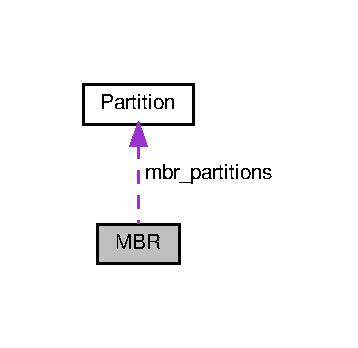
\includegraphics[width=172pt]{structMBR__coll__graph}
\end{center}
\end{figure}
\subsection*{Public Attributes}
\begin{DoxyCompactItemize}
\item 
\mbox{\Hypertarget{structMBR_a68ccdc40e66056adc16b4cad23264283}\label{structMBR_a68ccdc40e66056adc16b4cad23264283}} 
int {\bfseries mbr\+\_\+tamano}
\item 
\mbox{\Hypertarget{structMBR_a0c163e882325142b926667027d6b5546}\label{structMBR_a0c163e882325142b926667027d6b5546}} 
time\+\_\+t {\bfseries mbr\+\_\+fecha\+\_\+creacion}
\item 
\mbox{\Hypertarget{structMBR_a42f72f0002351e20fbeeef14f56e4bc6}\label{structMBR_a42f72f0002351e20fbeeef14f56e4bc6}} 
int {\bfseries mbr\+\_\+disk\+\_\+signature}
\item 
\mbox{\Hypertarget{structMBR_a984498f1082d2f067ae2acb5e9394c0c}\label{structMBR_a984498f1082d2f067ae2acb5e9394c0c}} 
char {\bfseries disk\+\_\+fit}
\item 
\mbox{\Hypertarget{structMBR_acd74d7b646ff5c0d2bdac6c001dc2129}\label{structMBR_acd74d7b646ff5c0d2bdac6c001dc2129}} 
\hyperlink{structPartition}{Partition} {\bfseries mbr\+\_\+partitions} \mbox{[}4\mbox{]}
\end{DoxyCompactItemize}


\subsection{Detailed Description}
Master boot record, sirve para administrar la memoria distribuida a las particiones a manera de meta data. 

The documentation for this struct was generated from the following file\+:\begin{DoxyCompactItemize}
\item 
structs.\+h\end{DoxyCompactItemize}

\hypertarget{classMKDISK__}{}\section{M\+K\+D\+I\+S\+K\+\_\+ Class Reference}
\label{classMKDISK__}\index{M\+K\+D\+I\+S\+K\+\_\+@{M\+K\+D\+I\+S\+K\+\_\+}}
\subsection*{Public Member Functions}
\begin{DoxyCompactItemize}
\item 
\hyperlink{classMKDISK___a320ed310d37d0912e1d96000213aed35}{M\+K\+D\+I\+S\+K\+\_\+} ()
\begin{DoxyCompactList}\small\item\em \hyperlink{structMBR}{M\+BR} auxiliar para escribir en disco. \end{DoxyCompactList}\item 
void \hyperlink{classMKDISK___a6fdf50f3e20009c7a84f3311ba1bc70c}{set\+Size} (char $\ast$size)
\item 
void \hyperlink{classMKDISK___a12001e69efc0110fafe2a5190d06a47d}{set\+Fit} (char $\ast$fit)
\item 
void \hyperlink{classMKDISK___a7a7755430182c5668dbbacf102df839d}{set\+Unit} (char $\ast$unit)
\item 
void \hyperlink{classMKDISK___ab46a4029dc7384bf7687c71221139a38}{set\+Path} (char $\ast$path)
\item 
void \hyperlink{classMKDISK___a9bcda3d3c6b9e0b6e42ff23538993378}{set\+Correct} ()
\item 
void \hyperlink{classMKDISK___a0589ffca3e13a4175510e2c6a60f2108}{print\+Mk} ()
\item 
int \hyperlink{classMKDISK___a6e61f79331a9d7d64f90791ec4f071c2}{create\+Disk} ()
\item 
int \hyperlink{classMKDISK___a2e73ce9adcd4ff071099420917d4585a}{get\+Size} ()
\item 
int \hyperlink{classMKDISK___a1dd09004e54bd40d98db5edcd7c62f61}{get\+Unit} ()
\item 
std\+::string \hyperlink{classMKDISK___a79ea3d7a98d06a929418dad2cd380523}{to\+Lower\+String} (string cadena)
\item 
void \hyperlink{classMKDISK___a7eee0fd7b056178946930a5e6bedf643}{configure\+Master} ()
\item 
char \hyperlink{classMKDISK___a7f632d7a17f80e97a0e4050c29ae95cd}{get\+Fit} ()
\end{DoxyCompactItemize}


\subsection{Constructor \& Destructor Documentation}
\mbox{\Hypertarget{classMKDISK___a320ed310d37d0912e1d96000213aed35}\label{classMKDISK___a320ed310d37d0912e1d96000213aed35}} 
\index{M\+K\+D\+I\+S\+K\+\_\+@{M\+K\+D\+I\+S\+K\+\_\+}!M\+K\+D\+I\+S\+K\+\_\+@{M\+K\+D\+I\+S\+K\+\_\+}}
\index{M\+K\+D\+I\+S\+K\+\_\+@{M\+K\+D\+I\+S\+K\+\_\+}!M\+K\+D\+I\+S\+K\+\_\+@{M\+K\+D\+I\+S\+K\+\_\+}}
\subsubsection{\texorpdfstring{M\+K\+D\+I\+S\+K\+\_\+()}{MKDISK\_()}}
{\footnotesize\ttfamily M\+K\+D\+I\+S\+K\+\_\+\+::\+M\+K\+D\+I\+S\+K\+\_\+ (\begin{DoxyParamCaption}{ }\end{DoxyParamCaption})\hspace{0.3cm}{\ttfamily [inline]}}



\hyperlink{structMBR}{M\+BR} auxiliar para escribir en disco. 

Constructor 

\subsection{Member Function Documentation}
\mbox{\Hypertarget{classMKDISK___a7eee0fd7b056178946930a5e6bedf643}\label{classMKDISK___a7eee0fd7b056178946930a5e6bedf643}} 
\index{M\+K\+D\+I\+S\+K\+\_\+@{M\+K\+D\+I\+S\+K\+\_\+}!configure\+Master@{configure\+Master}}
\index{configure\+Master@{configure\+Master}!M\+K\+D\+I\+S\+K\+\_\+@{M\+K\+D\+I\+S\+K\+\_\+}}
\subsubsection{\texorpdfstring{configure\+Master()}{configureMaster()}}
{\footnotesize\ttfamily void M\+K\+D\+I\+S\+K\+\_\+\+::configure\+Master (\begin{DoxyParamCaption}{ }\end{DoxyParamCaption})}

Configura el \hyperlink{structMBR}{M\+BR} cuando todos los parámetros están ok, este utiliza los parámetros de la clase misma por lo cual no recibe parámetros. Seteando tamaño

Seteando fecha y hora

Firma del disco

Guardando tipo de fit \mbox{\Hypertarget{classMKDISK___a6e61f79331a9d7d64f90791ec4f071c2}\label{classMKDISK___a6e61f79331a9d7d64f90791ec4f071c2}} 
\index{M\+K\+D\+I\+S\+K\+\_\+@{M\+K\+D\+I\+S\+K\+\_\+}!create\+Disk@{create\+Disk}}
\index{create\+Disk@{create\+Disk}!M\+K\+D\+I\+S\+K\+\_\+@{M\+K\+D\+I\+S\+K\+\_\+}}
\subsubsection{\texorpdfstring{create\+Disk()}{createDisk()}}
{\footnotesize\ttfamily int M\+K\+D\+I\+S\+K\+\_\+\+::create\+Disk (\begin{DoxyParamCaption}{ }\end{DoxyParamCaption})}

Crea un disco con los parámetros de la clase si todo está ok. Creando el disco principal

Comando para permisos.

Creando R\+A\+ID

Mensaje para notificar. \mbox{\Hypertarget{classMKDISK___a7f632d7a17f80e97a0e4050c29ae95cd}\label{classMKDISK___a7f632d7a17f80e97a0e4050c29ae95cd}} 
\index{M\+K\+D\+I\+S\+K\+\_\+@{M\+K\+D\+I\+S\+K\+\_\+}!get\+Fit@{get\+Fit}}
\index{get\+Fit@{get\+Fit}!M\+K\+D\+I\+S\+K\+\_\+@{M\+K\+D\+I\+S\+K\+\_\+}}
\subsubsection{\texorpdfstring{get\+Fit()}{getFit()}}
{\footnotesize\ttfamily char M\+K\+D\+I\+S\+K\+\_\+\+::get\+Fit (\begin{DoxyParamCaption}{ }\end{DoxyParamCaption})}

Obtiene la letra representativa del tipo de ajuste que se tiene. \mbox{\Hypertarget{classMKDISK___a2e73ce9adcd4ff071099420917d4585a}\label{classMKDISK___a2e73ce9adcd4ff071099420917d4585a}} 
\index{M\+K\+D\+I\+S\+K\+\_\+@{M\+K\+D\+I\+S\+K\+\_\+}!get\+Size@{get\+Size}}
\index{get\+Size@{get\+Size}!M\+K\+D\+I\+S\+K\+\_\+@{M\+K\+D\+I\+S\+K\+\_\+}}
\subsubsection{\texorpdfstring{get\+Size()}{getSize()}}
{\footnotesize\ttfamily int M\+K\+D\+I\+S\+K\+\_\+\+::get\+Size (\begin{DoxyParamCaption}{ }\end{DoxyParamCaption})}

Devuelve el tamaño del disco en bytes. \mbox{\Hypertarget{classMKDISK___a1dd09004e54bd40d98db5edcd7c62f61}\label{classMKDISK___a1dd09004e54bd40d98db5edcd7c62f61}} 
\index{M\+K\+D\+I\+S\+K\+\_\+@{M\+K\+D\+I\+S\+K\+\_\+}!get\+Unit@{get\+Unit}}
\index{get\+Unit@{get\+Unit}!M\+K\+D\+I\+S\+K\+\_\+@{M\+K\+D\+I\+S\+K\+\_\+}}
\subsubsection{\texorpdfstring{get\+Unit()}{getUnit()}}
{\footnotesize\ttfamily int M\+K\+D\+I\+S\+K\+\_\+\+::get\+Unit (\begin{DoxyParamCaption}{ }\end{DoxyParamCaption})}

Devuelve un múltiplo para cuantificar las unidades establecidas. \mbox{\Hypertarget{classMKDISK___a0589ffca3e13a4175510e2c6a60f2108}\label{classMKDISK___a0589ffca3e13a4175510e2c6a60f2108}} 
\index{M\+K\+D\+I\+S\+K\+\_\+@{M\+K\+D\+I\+S\+K\+\_\+}!print\+Mk@{print\+Mk}}
\index{print\+Mk@{print\+Mk}!M\+K\+D\+I\+S\+K\+\_\+@{M\+K\+D\+I\+S\+K\+\_\+}}
\subsubsection{\texorpdfstring{print\+Mk()}{printMk()}}
{\footnotesize\ttfamily void M\+K\+D\+I\+S\+K\+\_\+\+::print\+Mk (\begin{DoxyParamCaption}{ }\end{DoxyParamCaption})}

Acciona el comando para crear disco. \mbox{\Hypertarget{classMKDISK___a9bcda3d3c6b9e0b6e42ff23538993378}\label{classMKDISK___a9bcda3d3c6b9e0b6e42ff23538993378}} 
\index{M\+K\+D\+I\+S\+K\+\_\+@{M\+K\+D\+I\+S\+K\+\_\+}!set\+Correct@{set\+Correct}}
\index{set\+Correct@{set\+Correct}!M\+K\+D\+I\+S\+K\+\_\+@{M\+K\+D\+I\+S\+K\+\_\+}}
\subsubsection{\texorpdfstring{set\+Correct()}{setCorrect()}}
{\footnotesize\ttfamily void M\+K\+D\+I\+S\+K\+\_\+\+::set\+Correct (\begin{DoxyParamCaption}{ }\end{DoxyParamCaption})}

Verifica si la semántica del caso es adecuada. \mbox{\Hypertarget{classMKDISK___a12001e69efc0110fafe2a5190d06a47d}\label{classMKDISK___a12001e69efc0110fafe2a5190d06a47d}} 
\index{M\+K\+D\+I\+S\+K\+\_\+@{M\+K\+D\+I\+S\+K\+\_\+}!set\+Fit@{set\+Fit}}
\index{set\+Fit@{set\+Fit}!M\+K\+D\+I\+S\+K\+\_\+@{M\+K\+D\+I\+S\+K\+\_\+}}
\subsubsection{\texorpdfstring{set\+Fit()}{setFit()}}
{\footnotesize\ttfamily void M\+K\+D\+I\+S\+K\+\_\+\+::set\+Fit (\begin{DoxyParamCaption}\item[{char $\ast$}]{fit }\end{DoxyParamCaption})}

Configura el parámetro fit 
\begin{DoxyParams}{Parameters}
{\em fit} & Indica el tipo de ajuste con el que se agregarán las particiones en el disco. \\
\hline
\end{DoxyParams}
\mbox{\Hypertarget{classMKDISK___ab46a4029dc7384bf7687c71221139a38}\label{classMKDISK___ab46a4029dc7384bf7687c71221139a38}} 
\index{M\+K\+D\+I\+S\+K\+\_\+@{M\+K\+D\+I\+S\+K\+\_\+}!set\+Path@{set\+Path}}
\index{set\+Path@{set\+Path}!M\+K\+D\+I\+S\+K\+\_\+@{M\+K\+D\+I\+S\+K\+\_\+}}
\subsubsection{\texorpdfstring{set\+Path()}{setPath()}}
{\footnotesize\ttfamily void M\+K\+D\+I\+S\+K\+\_\+\+::set\+Path (\begin{DoxyParamCaption}\item[{char $\ast$}]{path }\end{DoxyParamCaption})}

Indica la ruta del archivo 
\begin{DoxyParams}{Parameters}
{\em path} & indica en donde se debe de crear el disco. \\
\hline
\end{DoxyParams}
\mbox{\Hypertarget{classMKDISK___a6fdf50f3e20009c7a84f3311ba1bc70c}\label{classMKDISK___a6fdf50f3e20009c7a84f3311ba1bc70c}} 
\index{M\+K\+D\+I\+S\+K\+\_\+@{M\+K\+D\+I\+S\+K\+\_\+}!set\+Size@{set\+Size}}
\index{set\+Size@{set\+Size}!M\+K\+D\+I\+S\+K\+\_\+@{M\+K\+D\+I\+S\+K\+\_\+}}
\subsubsection{\texorpdfstring{set\+Size()}{setSize()}}
{\footnotesize\ttfamily void M\+K\+D\+I\+S\+K\+\_\+\+::set\+Size (\begin{DoxyParamCaption}\item[{char $\ast$}]{size }\end{DoxyParamCaption})}

Configura el atributo size 
\begin{DoxyParams}{Parameters}
{\em size} & Indica la cantidad de unidades que ocupará el disco. \\
\hline
\end{DoxyParams}
\mbox{\Hypertarget{classMKDISK___a7a7755430182c5668dbbacf102df839d}\label{classMKDISK___a7a7755430182c5668dbbacf102df839d}} 
\index{M\+K\+D\+I\+S\+K\+\_\+@{M\+K\+D\+I\+S\+K\+\_\+}!set\+Unit@{set\+Unit}}
\index{set\+Unit@{set\+Unit}!M\+K\+D\+I\+S\+K\+\_\+@{M\+K\+D\+I\+S\+K\+\_\+}}
\subsubsection{\texorpdfstring{set\+Unit()}{setUnit()}}
{\footnotesize\ttfamily void M\+K\+D\+I\+S\+K\+\_\+\+::set\+Unit (\begin{DoxyParamCaption}\item[{char $\ast$}]{unit }\end{DoxyParamCaption})}

Configura las unidades del disco. 
\begin{DoxyParams}{Parameters}
{\em unit} & indica si son megabytes, kilobytes ó bytes. \\
\hline
\end{DoxyParams}
\mbox{\Hypertarget{classMKDISK___a79ea3d7a98d06a929418dad2cd380523}\label{classMKDISK___a79ea3d7a98d06a929418dad2cd380523}} 
\index{M\+K\+D\+I\+S\+K\+\_\+@{M\+K\+D\+I\+S\+K\+\_\+}!to\+Lower\+String@{to\+Lower\+String}}
\index{to\+Lower\+String@{to\+Lower\+String}!M\+K\+D\+I\+S\+K\+\_\+@{M\+K\+D\+I\+S\+K\+\_\+}}
\subsubsection{\texorpdfstring{to\+Lower\+String()}{toLowerString()}}
{\footnotesize\ttfamily string M\+K\+D\+I\+S\+K\+\_\+\+::to\+Lower\+String (\begin{DoxyParamCaption}\item[{string}]{cadena }\end{DoxyParamCaption})}

Devuelve un string con todos los cáracteres contenidos en el parámetro en minúscula. 
\begin{DoxyParams}{Parameters}
{\em cadena} & Cadena que se desea en minúsculas. \\
\hline
\end{DoxyParams}


The documentation for this class was generated from the following file\+:\begin{DoxyCompactItemize}
\item 
M\+K\+D\+I\+S\+K.\+h\end{DoxyCompactItemize}

\hypertarget{classMOUNT__}{}\section{M\+O\+U\+N\+T\+\_\+ Class Reference}
\label{classMOUNT__}\index{M\+O\+U\+N\+T\+\_\+@{M\+O\+U\+N\+T\+\_\+}}
\subsection*{Public Member Functions}
\begin{DoxyCompactItemize}
\item 
\hyperlink{classMOUNT___ab2412abd1fe27e4c58bad1ec543c1bfd}{M\+O\+U\+N\+T\+\_\+} ()
\begin{DoxyCompactList}\small\item\em Semántica correcta de la función. \end{DoxyCompactList}\item 
void \hyperlink{classMOUNT___a6d628a264a4f7652fb79db60a8f74d5c}{set\+Path} (char $\ast$c)
\item 
void \hyperlink{classMOUNT___a07920ca266d5f28996f14ac76d5cfbd4}{set\+Name} (char $\ast$c)
\item 
void \hyperlink{classMOUNT___a938fb0ea2d4dacaf795ceed3dba82552}{set\+Id} ()
\item 
void \hyperlink{classMOUNT___a0c2649414eda3ba4132e847e9903830c}{set\+Letter} (char c)
\item 
string \hyperlink{classMOUNT___aa22dd1507def0dd79278528eb364ff2e}{get\+Name} ()
\item 
string \hyperlink{classMOUNT___a3fa81be2f40ddf3f043c8f459cbaa3e6}{get\+Path} ()
\item 
char \hyperlink{classMOUNT___ac5af7651aa4eeede67b21c1c728bf898}{get\+Letter} ()
\item 
int \hyperlink{classMOUNT___a737ec85f4dd23d389d85b9dee48d18ce}{get\+Number} ()
\item 
string \hyperlink{classMOUNT___ae42ec4c474c9fd74a25869cf13f9436a}{get\+Id} ()
\item 
\mbox{\Hypertarget{classMOUNT___adef287e870112d76ef9e03e79c95c518}\label{classMOUNT___adef287e870112d76ef9e03e79c95c518}} 
string {\bfseries conf\+Id} ()
\item 
void \hyperlink{classMOUNT___ae0df247d4a3d27886c941352607d7bc2}{semantic} ()
\item 
void \hyperlink{classMOUNT___a4ed2206e1edd2eec7804514ebdbb8ee3}{run} ()
\item 
int \hyperlink{classMOUNT___a3ff41f627cb6e3e573da1b627850e01a}{part\+Index} ()
\item 
int \hyperlink{classMOUNT___a709e81cf0e777d2dfa9c24ca30a3c778}{Logic\+Part\+Index} ()
\item 
void \hyperlink{classMOUNT___a58750b67c92586b45a944d5eeb2f7645}{mount\+Partition} ()
\item 
\mbox{\Hypertarget{classMOUNT___adb6c42535a48b023d8e5f5afed030781}\label{classMOUNT___adb6c42535a48b023d8e5f5afed030781}} 
bool {\bfseries is\+Mounted} ()
\end{DoxyCompactItemize}


\subsection{Constructor \& Destructor Documentation}
\mbox{\Hypertarget{classMOUNT___ab2412abd1fe27e4c58bad1ec543c1bfd}\label{classMOUNT___ab2412abd1fe27e4c58bad1ec543c1bfd}} 
\index{M\+O\+U\+N\+T\+\_\+@{M\+O\+U\+N\+T\+\_\+}!M\+O\+U\+N\+T\+\_\+@{M\+O\+U\+N\+T\+\_\+}}
\index{M\+O\+U\+N\+T\+\_\+@{M\+O\+U\+N\+T\+\_\+}!M\+O\+U\+N\+T\+\_\+@{M\+O\+U\+N\+T\+\_\+}}
\subsubsection{\texorpdfstring{M\+O\+U\+N\+T\+\_\+()}{MOUNT\_()}}
{\footnotesize\ttfamily M\+O\+U\+N\+T\+\_\+\+::\+M\+O\+U\+N\+T\+\_\+ (\begin{DoxyParamCaption}{ }\end{DoxyParamCaption})\hspace{0.3cm}{\ttfamily [inline]}}



Semántica correcta de la función. 

Constructor de M\+O\+U\+NT 

\subsection{Member Function Documentation}
\mbox{\Hypertarget{classMOUNT___ae42ec4c474c9fd74a25869cf13f9436a}\label{classMOUNT___ae42ec4c474c9fd74a25869cf13f9436a}} 
\index{M\+O\+U\+N\+T\+\_\+@{M\+O\+U\+N\+T\+\_\+}!get\+Id@{get\+Id}}
\index{get\+Id@{get\+Id}!M\+O\+U\+N\+T\+\_\+@{M\+O\+U\+N\+T\+\_\+}}
\subsubsection{\texorpdfstring{get\+Id()}{getId()}}
{\footnotesize\ttfamily string M\+O\+U\+N\+T\+\_\+\+::get\+Id (\begin{DoxyParamCaption}{ }\end{DoxyParamCaption})}

Calcula el id mediante la concatenacion de VD + letra del disco + número de partición de ese disco. \mbox{\Hypertarget{classMOUNT___ac5af7651aa4eeede67b21c1c728bf898}\label{classMOUNT___ac5af7651aa4eeede67b21c1c728bf898}} 
\index{M\+O\+U\+N\+T\+\_\+@{M\+O\+U\+N\+T\+\_\+}!get\+Letter@{get\+Letter}}
\index{get\+Letter@{get\+Letter}!M\+O\+U\+N\+T\+\_\+@{M\+O\+U\+N\+T\+\_\+}}
\subsubsection{\texorpdfstring{get\+Letter()}{getLetter()}}
{\footnotesize\ttfamily char M\+O\+U\+N\+T\+\_\+\+::get\+Letter (\begin{DoxyParamCaption}{ }\end{DoxyParamCaption})}

Calcula la letra del disco a la cual pertenece la partición \mbox{\Hypertarget{classMOUNT___aa22dd1507def0dd79278528eb364ff2e}\label{classMOUNT___aa22dd1507def0dd79278528eb364ff2e}} 
\index{M\+O\+U\+N\+T\+\_\+@{M\+O\+U\+N\+T\+\_\+}!get\+Name@{get\+Name}}
\index{get\+Name@{get\+Name}!M\+O\+U\+N\+T\+\_\+@{M\+O\+U\+N\+T\+\_\+}}
\subsubsection{\texorpdfstring{get\+Name()}{getName()}}
{\footnotesize\ttfamily string M\+O\+U\+N\+T\+\_\+\+::get\+Name (\begin{DoxyParamCaption}{ }\end{DoxyParamCaption})\hspace{0.3cm}{\ttfamily [inline]}}

Obtiene el nombre de la partición \mbox{\Hypertarget{classMOUNT___a737ec85f4dd23d389d85b9dee48d18ce}\label{classMOUNT___a737ec85f4dd23d389d85b9dee48d18ce}} 
\index{M\+O\+U\+N\+T\+\_\+@{M\+O\+U\+N\+T\+\_\+}!get\+Number@{get\+Number}}
\index{get\+Number@{get\+Number}!M\+O\+U\+N\+T\+\_\+@{M\+O\+U\+N\+T\+\_\+}}
\subsubsection{\texorpdfstring{get\+Number()}{getNumber()}}
{\footnotesize\ttfamily int M\+O\+U\+N\+T\+\_\+\+::get\+Number (\begin{DoxyParamCaption}{ }\end{DoxyParamCaption})}

Obtiene el número de partición montada de un mismo disco. \mbox{\Hypertarget{classMOUNT___a3fa81be2f40ddf3f043c8f459cbaa3e6}\label{classMOUNT___a3fa81be2f40ddf3f043c8f459cbaa3e6}} 
\index{M\+O\+U\+N\+T\+\_\+@{M\+O\+U\+N\+T\+\_\+}!get\+Path@{get\+Path}}
\index{get\+Path@{get\+Path}!M\+O\+U\+N\+T\+\_\+@{M\+O\+U\+N\+T\+\_\+}}
\subsubsection{\texorpdfstring{get\+Path()}{getPath()}}
{\footnotesize\ttfamily string M\+O\+U\+N\+T\+\_\+\+::get\+Path (\begin{DoxyParamCaption}{ }\end{DoxyParamCaption})\hspace{0.3cm}{\ttfamily [inline]}}

Retorna la ruta del disco de esta partición. \mbox{\Hypertarget{classMOUNT___a709e81cf0e777d2dfa9c24ca30a3c778}\label{classMOUNT___a709e81cf0e777d2dfa9c24ca30a3c778}} 
\index{M\+O\+U\+N\+T\+\_\+@{M\+O\+U\+N\+T\+\_\+}!Logic\+Part\+Index@{Logic\+Part\+Index}}
\index{Logic\+Part\+Index@{Logic\+Part\+Index}!M\+O\+U\+N\+T\+\_\+@{M\+O\+U\+N\+T\+\_\+}}
\subsubsection{\texorpdfstring{Logic\+Part\+Index()}{LogicPartIndex()}}
{\footnotesize\ttfamily int M\+O\+U\+N\+T\+\_\+\+::\+Logic\+Part\+Index (\begin{DoxyParamCaption}{ }\end{DoxyParamCaption})}

Obtiene el indice de partición en donde está almacenada la lógica. Buscar la partición extendida del disco

Buscar si existe una lógica en el disco \mbox{\Hypertarget{classMOUNT___a58750b67c92586b45a944d5eeb2f7645}\label{classMOUNT___a58750b67c92586b45a944d5eeb2f7645}} 
\index{M\+O\+U\+N\+T\+\_\+@{M\+O\+U\+N\+T\+\_\+}!mount\+Partition@{mount\+Partition}}
\index{mount\+Partition@{mount\+Partition}!M\+O\+U\+N\+T\+\_\+@{M\+O\+U\+N\+T\+\_\+}}
\subsubsection{\texorpdfstring{mount\+Partition()}{mountPartition()}}
{\footnotesize\ttfamily void M\+O\+U\+N\+T\+\_\+\+::mount\+Partition (\begin{DoxyParamCaption}{ }\end{DoxyParamCaption})}

Abrir el archivo

Cambiar su status

Reescribirlo

Verificar si está montada

Insertar a la lista.

Leer el ebr

Cambiar su estado a montado.

Insertar a la lista. \mbox{\Hypertarget{classMOUNT___a3ff41f627cb6e3e573da1b627850e01a}\label{classMOUNT___a3ff41f627cb6e3e573da1b627850e01a}} 
\index{M\+O\+U\+N\+T\+\_\+@{M\+O\+U\+N\+T\+\_\+}!part\+Index@{part\+Index}}
\index{part\+Index@{part\+Index}!M\+O\+U\+N\+T\+\_\+@{M\+O\+U\+N\+T\+\_\+}}
\subsubsection{\texorpdfstring{part\+Index()}{partIndex()}}
{\footnotesize\ttfamily int M\+O\+U\+N\+T\+\_\+\+::part\+Index (\begin{DoxyParamCaption}{ }\end{DoxyParamCaption})}

Obtiene el indice de partición que tiene la deseada en el disco. \mbox{\Hypertarget{classMOUNT___a4ed2206e1edd2eec7804514ebdbb8ee3}\label{classMOUNT___a4ed2206e1edd2eec7804514ebdbb8ee3}} 
\index{M\+O\+U\+N\+T\+\_\+@{M\+O\+U\+N\+T\+\_\+}!run@{run}}
\index{run@{run}!M\+O\+U\+N\+T\+\_\+@{M\+O\+U\+N\+T\+\_\+}}
\subsubsection{\texorpdfstring{run()}{run()}}
{\footnotesize\ttfamily void M\+O\+U\+N\+T\+\_\+\+::run (\begin{DoxyParamCaption}{ }\end{DoxyParamCaption})}

Ejecuta la montura. \mbox{\Hypertarget{classMOUNT___ae0df247d4a3d27886c941352607d7bc2}\label{classMOUNT___ae0df247d4a3d27886c941352607d7bc2}} 
\index{M\+O\+U\+N\+T\+\_\+@{M\+O\+U\+N\+T\+\_\+}!semantic@{semantic}}
\index{semantic@{semantic}!M\+O\+U\+N\+T\+\_\+@{M\+O\+U\+N\+T\+\_\+}}
\subsubsection{\texorpdfstring{semantic()}{semantic()}}
{\footnotesize\ttfamily void M\+O\+U\+N\+T\+\_\+\+::semantic (\begin{DoxyParamCaption}{ }\end{DoxyParamCaption})}

Verifica la semántica de la operación ingresada en consola. \mbox{\Hypertarget{classMOUNT___a938fb0ea2d4dacaf795ceed3dba82552}\label{classMOUNT___a938fb0ea2d4dacaf795ceed3dba82552}} 
\index{M\+O\+U\+N\+T\+\_\+@{M\+O\+U\+N\+T\+\_\+}!set\+Id@{set\+Id}}
\index{set\+Id@{set\+Id}!M\+O\+U\+N\+T\+\_\+@{M\+O\+U\+N\+T\+\_\+}}
\subsubsection{\texorpdfstring{set\+Id()}{setId()}}
{\footnotesize\ttfamily void M\+O\+U\+N\+T\+\_\+\+::set\+Id (\begin{DoxyParamCaption}{ }\end{DoxyParamCaption})}

Guarda el id que se le asigno a la partición en la lista de montadas. \mbox{\Hypertarget{classMOUNT___a0c2649414eda3ba4132e847e9903830c}\label{classMOUNT___a0c2649414eda3ba4132e847e9903830c}} 
\index{M\+O\+U\+N\+T\+\_\+@{M\+O\+U\+N\+T\+\_\+}!set\+Letter@{set\+Letter}}
\index{set\+Letter@{set\+Letter}!M\+O\+U\+N\+T\+\_\+@{M\+O\+U\+N\+T\+\_\+}}
\subsubsection{\texorpdfstring{set\+Letter()}{setLetter()}}
{\footnotesize\ttfamily void M\+O\+U\+N\+T\+\_\+\+::set\+Letter (\begin{DoxyParamCaption}\item[{char}]{c }\end{DoxyParamCaption})}

Guarda la letra del disco a la que pertenece esta partición montada. 
\begin{DoxyParams}{Parameters}
{\em c} & letra asignada por el sistema de montaje a su disco. \\
\hline
\end{DoxyParams}
\mbox{\Hypertarget{classMOUNT___a07920ca266d5f28996f14ac76d5cfbd4}\label{classMOUNT___a07920ca266d5f28996f14ac76d5cfbd4}} 
\index{M\+O\+U\+N\+T\+\_\+@{M\+O\+U\+N\+T\+\_\+}!set\+Name@{set\+Name}}
\index{set\+Name@{set\+Name}!M\+O\+U\+N\+T\+\_\+@{M\+O\+U\+N\+T\+\_\+}}
\subsubsection{\texorpdfstring{set\+Name()}{setName()}}
{\footnotesize\ttfamily void M\+O\+U\+N\+T\+\_\+\+::set\+Name (\begin{DoxyParamCaption}\item[{char $\ast$}]{c }\end{DoxyParamCaption})\hspace{0.3cm}{\ttfamily [inline]}}

Guarda el nombre de la partición a montar. 
\begin{DoxyParams}{Parameters}
{\em c} & partición a montar. \\
\hline
\end{DoxyParams}
\mbox{\Hypertarget{classMOUNT___a6d628a264a4f7652fb79db60a8f74d5c}\label{classMOUNT___a6d628a264a4f7652fb79db60a8f74d5c}} 
\index{M\+O\+U\+N\+T\+\_\+@{M\+O\+U\+N\+T\+\_\+}!set\+Path@{set\+Path}}
\index{set\+Path@{set\+Path}!M\+O\+U\+N\+T\+\_\+@{M\+O\+U\+N\+T\+\_\+}}
\subsubsection{\texorpdfstring{set\+Path()}{setPath()}}
{\footnotesize\ttfamily void M\+O\+U\+N\+T\+\_\+\+::set\+Path (\begin{DoxyParamCaption}\item[{char $\ast$}]{c }\end{DoxyParamCaption})\hspace{0.3cm}{\ttfamily [inline]}}

Guarda el valor de la ruta 
\begin{DoxyParams}{Parameters}
{\em c} & indica la ruta del disco de la partición a montar. \\
\hline
\end{DoxyParams}


The documentation for this class was generated from the following file\+:\begin{DoxyCompactItemize}
\item 
M\+O\+U\+N\+T.\+h\end{DoxyCompactItemize}

\hypertarget{structPartition}{}\section{Partition Struct Reference}
\label{structPartition}\index{Partition@{Partition}}


{\ttfamily \#include $<$structs.\+h$>$}

\subsection*{Public Attributes}
\begin{DoxyCompactItemize}
\item 
\mbox{\Hypertarget{structPartition_a2d12cff678829bd670c6ae3a49ed04a6}\label{structPartition_a2d12cff678829bd670c6ae3a49ed04a6}} 
char {\bfseries part\+\_\+status} = \textquotesingle{}0\textquotesingle{}
\item 
\mbox{\Hypertarget{structPartition_afe3fef54e52e839f3f153c6d2a4f932e}\label{structPartition_afe3fef54e52e839f3f153c6d2a4f932e}} 
char {\bfseries part\+\_\+type} = \textquotesingle{}0\textquotesingle{}
\item 
\mbox{\Hypertarget{structPartition_a6232bfa1f2f926b88ae704562283fc98}\label{structPartition_a6232bfa1f2f926b88ae704562283fc98}} 
char {\bfseries part\+\_\+fit} = \textquotesingle{}0\textquotesingle{}
\item 
\mbox{\Hypertarget{structPartition_a81300df85aef6c01b6d87938da973030}\label{structPartition_a81300df85aef6c01b6d87938da973030}} 
int {\bfseries part\+\_\+start} = -\/1
\item 
\mbox{\Hypertarget{structPartition_a76ba8d57b0c043332e156bd1c57b774c}\label{structPartition_a76ba8d57b0c043332e156bd1c57b774c}} 
int {\bfseries part\+\_\+size} = 0
\item 
\mbox{\Hypertarget{structPartition_a737c9efae493f96a75693b6417dec937}\label{structPartition_a737c9efae493f96a75693b6417dec937}} 
char {\bfseries part\+\_\+name} \mbox{[}16\mbox{]} = \char`\"{}\char`\"{}
\end{DoxyCompactItemize}


\subsection{Detailed Description}
Structs que son útiles para llevar un manejo lógico de la memoria. Particiones primarias. 

The documentation for this struct was generated from the following file\+:\begin{DoxyCompactItemize}
\item 
structs.\+h\end{DoxyCompactItemize}

\hypertarget{classREP__}{}\section{R\+E\+P\+\_\+ Class Reference}
\label{classREP__}\index{R\+E\+P\+\_\+@{R\+E\+P\+\_\+}}
\subsection*{Public Member Functions}
\begin{DoxyCompactItemize}
\item 
\hyperlink{classREP___a067733aa62d5f5cc028fd4de7e2eba3a}{R\+E\+P\+\_\+} ()
\begin{DoxyCompactList}\small\item\em Indica si la partición que se desea está montada. \end{DoxyCompactList}\item 
void \hyperlink{classREP___a42631749f8e85ecee3d125f2db1167f0}{set\+Id} (char $\ast$id)
\item 
void \hyperlink{classREP___aad647454ea8a5ef1d8b962f785af7bb8}{set\+Path} (char $\ast$path)
\item 
void \hyperlink{classREP___ac10352477beb170b15096cf13c559935}{conf\+Ruta} ()
\item 
void \hyperlink{classREP___a6e13e906980b5ee0d3eb87021f3b73b9}{set\+Ruta} (char $\ast$ruta)
\item 
void \hyperlink{classREP___ad66a2155dafd5a9ca0cec161e42ddd3e}{set\+Name} (char $\ast$name)
\item 
\mbox{\Hypertarget{classREP___ab5c3e45ded785eaeac191f6ecbf8b042}\label{classREP___ab5c3e45ded785eaeac191f6ecbf8b042}} 
char $\ast$ {\bfseries get\+Id} ()
\item 
\mbox{\Hypertarget{classREP___aa5303ed9e76c35cb81e751dea99389c5}\label{classREP___aa5303ed9e76c35cb81e751dea99389c5}} 
char $\ast$ {\bfseries get\+Ruta} ()
\item 
char $\ast$ \hyperlink{classREP___a9d4e00566ad8a08662f06e97265e059d}{get\+Name} ()
\item 
void \hyperlink{classREP___a7b6a615bdcab7164cddb336a4b0ef1b7}{semantic} ()
\item 
void \hyperlink{classREP___abe74de18a398b8f428e868a316bcec58}{run} ()
\item 
string \hyperlink{classREP___ae1d0fa6e478eac36a3246d73e574b9f2}{to\+Lower\+String} (string input)
\item 
void \hyperlink{classREP___aa1f6945c91d9494c42a0c34338a83790}{report\+M\+BR} ()
\item 
void \hyperlink{classREP___aa0429938785e2c916b3c89148a4d7317}{report\+D\+I\+SK} ()
\end{DoxyCompactItemize}


\subsection{Constructor \& Destructor Documentation}
\mbox{\Hypertarget{classREP___a067733aa62d5f5cc028fd4de7e2eba3a}\label{classREP___a067733aa62d5f5cc028fd4de7e2eba3a}} 
\index{R\+E\+P\+\_\+@{R\+E\+P\+\_\+}!R\+E\+P\+\_\+@{R\+E\+P\+\_\+}}
\index{R\+E\+P\+\_\+@{R\+E\+P\+\_\+}!R\+E\+P\+\_\+@{R\+E\+P\+\_\+}}
\subsubsection{\texorpdfstring{R\+E\+P\+\_\+()}{REP\_()}}
{\footnotesize\ttfamily R\+E\+P\+\_\+\+::\+R\+E\+P\+\_\+ (\begin{DoxyParamCaption}{ }\end{DoxyParamCaption})\hspace{0.3cm}{\ttfamily [inline]}}



Indica si la partición que se desea está montada. 

Constructor 

\subsection{Member Function Documentation}
\mbox{\Hypertarget{classREP___ac10352477beb170b15096cf13c559935}\label{classREP___ac10352477beb170b15096cf13c559935}} 
\index{R\+E\+P\+\_\+@{R\+E\+P\+\_\+}!conf\+Ruta@{conf\+Ruta}}
\index{conf\+Ruta@{conf\+Ruta}!R\+E\+P\+\_\+@{R\+E\+P\+\_\+}}
\subsubsection{\texorpdfstring{conf\+Ruta()}{confRuta()}}
{\footnotesize\ttfamily void R\+E\+P\+\_\+\+::conf\+Ruta (\begin{DoxyParamCaption}{ }\end{DoxyParamCaption})}

Configura la ruta en la que se guardará ya que se necesitan variantes para guardar el dot y para la imagen. \mbox{\Hypertarget{classREP___a9d4e00566ad8a08662f06e97265e059d}\label{classREP___a9d4e00566ad8a08662f06e97265e059d}} 
\index{R\+E\+P\+\_\+@{R\+E\+P\+\_\+}!get\+Name@{get\+Name}}
\index{get\+Name@{get\+Name}!R\+E\+P\+\_\+@{R\+E\+P\+\_\+}}
\subsubsection{\texorpdfstring{get\+Name()}{getName()}}
{\footnotesize\ttfamily char$\ast$ R\+E\+P\+\_\+\+::get\+Name (\begin{DoxyParamCaption}{ }\end{DoxyParamCaption})\hspace{0.3cm}{\ttfamily [inline]}}

Obtiene el nombre que se le dará al rerporte. \mbox{\Hypertarget{classREP___aa0429938785e2c916b3c89148a4d7317}\label{classREP___aa0429938785e2c916b3c89148a4d7317}} 
\index{R\+E\+P\+\_\+@{R\+E\+P\+\_\+}!report\+D\+I\+SK@{report\+D\+I\+SK}}
\index{report\+D\+I\+SK@{report\+D\+I\+SK}!R\+E\+P\+\_\+@{R\+E\+P\+\_\+}}
\subsubsection{\texorpdfstring{report\+D\+I\+S\+K()}{reportDISK()}}
{\footnotesize\ttfamily void R\+E\+P\+\_\+\+::report\+D\+I\+SK (\begin{DoxyParamCaption}{ }\end{DoxyParamCaption})}

Método para generar el reporte del disco \mbox{\Hypertarget{classREP___aa1f6945c91d9494c42a0c34338a83790}\label{classREP___aa1f6945c91d9494c42a0c34338a83790}} 
\index{R\+E\+P\+\_\+@{R\+E\+P\+\_\+}!report\+M\+BR@{report\+M\+BR}}
\index{report\+M\+BR@{report\+M\+BR}!R\+E\+P\+\_\+@{R\+E\+P\+\_\+}}
\subsubsection{\texorpdfstring{report\+M\+B\+R()}{reportMBR()}}
{\footnotesize\ttfamily void R\+E\+P\+\_\+\+::report\+M\+BR (\begin{DoxyParamCaption}{ }\end{DoxyParamCaption})}

Método para generar el reporte de \hyperlink{structMBR}{M\+BR} \mbox{\Hypertarget{classREP___abe74de18a398b8f428e868a316bcec58}\label{classREP___abe74de18a398b8f428e868a316bcec58}} 
\index{R\+E\+P\+\_\+@{R\+E\+P\+\_\+}!run@{run}}
\index{run@{run}!R\+E\+P\+\_\+@{R\+E\+P\+\_\+}}
\subsubsection{\texorpdfstring{run()}{run()}}
{\footnotesize\ttfamily void R\+E\+P\+\_\+\+::run (\begin{DoxyParamCaption}{ }\end{DoxyParamCaption})}

Método para ejecutar \mbox{\Hypertarget{classREP___a7b6a615bdcab7164cddb336a4b0ef1b7}\label{classREP___a7b6a615bdcab7164cddb336a4b0ef1b7}} 
\index{R\+E\+P\+\_\+@{R\+E\+P\+\_\+}!semantic@{semantic}}
\index{semantic@{semantic}!R\+E\+P\+\_\+@{R\+E\+P\+\_\+}}
\subsubsection{\texorpdfstring{semantic()}{semantic()}}
{\footnotesize\ttfamily void R\+E\+P\+\_\+\+::semantic (\begin{DoxyParamCaption}{ }\end{DoxyParamCaption})}

Método para verificar semántica de la operación \mbox{\Hypertarget{classREP___a42631749f8e85ecee3d125f2db1167f0}\label{classREP___a42631749f8e85ecee3d125f2db1167f0}} 
\index{R\+E\+P\+\_\+@{R\+E\+P\+\_\+}!set\+Id@{set\+Id}}
\index{set\+Id@{set\+Id}!R\+E\+P\+\_\+@{R\+E\+P\+\_\+}}
\subsubsection{\texorpdfstring{set\+Id()}{setId()}}
{\footnotesize\ttfamily void R\+E\+P\+\_\+\+::set\+Id (\begin{DoxyParamCaption}\item[{char $\ast$}]{id }\end{DoxyParamCaption})}

Configura el id de la partición montada a escribir. 
\begin{DoxyParams}{Parameters}
{\em id} & identificador de la partición montada en el sistema. \\
\hline
\end{DoxyParams}
\mbox{\Hypertarget{classREP___ad66a2155dafd5a9ca0cec161e42ddd3e}\label{classREP___ad66a2155dafd5a9ca0cec161e42ddd3e}} 
\index{R\+E\+P\+\_\+@{R\+E\+P\+\_\+}!set\+Name@{set\+Name}}
\index{set\+Name@{set\+Name}!R\+E\+P\+\_\+@{R\+E\+P\+\_\+}}
\subsubsection{\texorpdfstring{set\+Name()}{setName()}}
{\footnotesize\ttfamily void R\+E\+P\+\_\+\+::set\+Name (\begin{DoxyParamCaption}\item[{char $\ast$}]{name }\end{DoxyParamCaption})\hspace{0.3cm}{\ttfamily [inline]}}

Guarda el nombre de la partición montada que se reportará. 
\begin{DoxyParams}{Parameters}
{\em name} & indica el nombre de la partición en el sistema de particiones montadas. \\
\hline
\end{DoxyParams}
\mbox{\Hypertarget{classREP___aad647454ea8a5ef1d8b962f785af7bb8}\label{classREP___aad647454ea8a5ef1d8b962f785af7bb8}} 
\index{R\+E\+P\+\_\+@{R\+E\+P\+\_\+}!set\+Path@{set\+Path}}
\index{set\+Path@{set\+Path}!R\+E\+P\+\_\+@{R\+E\+P\+\_\+}}
\subsubsection{\texorpdfstring{set\+Path()}{setPath()}}
{\footnotesize\ttfamily void R\+E\+P\+\_\+\+::set\+Path (\begin{DoxyParamCaption}\item[{char $\ast$}]{path }\end{DoxyParamCaption})}

Configura la ruta en donde se guardará el reporte. 
\begin{DoxyParams}{Parameters}
{\em path} & ruta que se pretende guardar el reporte. \\
\hline
\end{DoxyParams}
\mbox{\Hypertarget{classREP___a6e13e906980b5ee0d3eb87021f3b73b9}\label{classREP___a6e13e906980b5ee0d3eb87021f3b73b9}} 
\index{R\+E\+P\+\_\+@{R\+E\+P\+\_\+}!set\+Ruta@{set\+Ruta}}
\index{set\+Ruta@{set\+Ruta}!R\+E\+P\+\_\+@{R\+E\+P\+\_\+}}
\subsubsection{\texorpdfstring{set\+Ruta()}{setRuta()}}
{\footnotesize\ttfamily void R\+E\+P\+\_\+\+::set\+Ruta (\begin{DoxyParamCaption}\item[{char $\ast$}]{ruta }\end{DoxyParamCaption})\hspace{0.3cm}{\ttfamily [inline]}}

Guarda el valor de la ruta 
\begin{DoxyParams}{Parameters}
{\em ruta} & dirección en la que se almacenará el reporte. \\
\hline
\end{DoxyParams}
\mbox{\Hypertarget{classREP___ae1d0fa6e478eac36a3246d73e574b9f2}\label{classREP___ae1d0fa6e478eac36a3246d73e574b9f2}} 
\index{R\+E\+P\+\_\+@{R\+E\+P\+\_\+}!to\+Lower\+String@{to\+Lower\+String}}
\index{to\+Lower\+String@{to\+Lower\+String}!R\+E\+P\+\_\+@{R\+E\+P\+\_\+}}
\subsubsection{\texorpdfstring{to\+Lower\+String()}{toLowerString()}}
{\footnotesize\ttfamily string R\+E\+P\+\_\+\+::to\+Lower\+String (\begin{DoxyParamCaption}\item[{string}]{input }\end{DoxyParamCaption})}

Método para convertir un string a minúsculas. 

The documentation for this class was generated from the following file\+:\begin{DoxyCompactItemize}
\item 
R\+E\+P.\+h\end{DoxyCompactItemize}

\hypertarget{classRMDISK__}{}\section{R\+M\+D\+I\+S\+K\+\_\+ Class Reference}
\label{classRMDISK__}\index{R\+M\+D\+I\+S\+K\+\_\+@{R\+M\+D\+I\+S\+K\+\_\+}}
\subsection*{Public Member Functions}
\begin{DoxyCompactItemize}
\item 
\hyperlink{classRMDISK___ad4e0a6a86ffc42b52cd98d039e035020}{R\+M\+D\+I\+S\+K\+\_\+} ()
\begin{DoxyCompactList}\small\item\em Indica semántica correcta. \end{DoxyCompactList}\item 
void \hyperlink{classRMDISK___a49d4ed7ede3b344f5be86dd411314d34}{borrar\+Disco} ()
\item 
void \hyperlink{classRMDISK___afe9e2e1e4ab06f37188e78fa5ce2e83b}{set\+Obligatoriedad} ()
\item 
void \hyperlink{classRMDISK___a0aca679d77aa2cef1a72568693814eb8}{set\+Path} (char $\ast$ruta)
\end{DoxyCompactItemize}


\subsection{Constructor \& Destructor Documentation}
\mbox{\Hypertarget{classRMDISK___ad4e0a6a86ffc42b52cd98d039e035020}\label{classRMDISK___ad4e0a6a86ffc42b52cd98d039e035020}} 
\index{R\+M\+D\+I\+S\+K\+\_\+@{R\+M\+D\+I\+S\+K\+\_\+}!R\+M\+D\+I\+S\+K\+\_\+@{R\+M\+D\+I\+S\+K\+\_\+}}
\index{R\+M\+D\+I\+S\+K\+\_\+@{R\+M\+D\+I\+S\+K\+\_\+}!R\+M\+D\+I\+S\+K\+\_\+@{R\+M\+D\+I\+S\+K\+\_\+}}
\subsubsection{\texorpdfstring{R\+M\+D\+I\+S\+K\+\_\+()}{RMDISK\_()}}
{\footnotesize\ttfamily R\+M\+D\+I\+S\+K\+\_\+\+::\+R\+M\+D\+I\+S\+K\+\_\+ (\begin{DoxyParamCaption}{ }\end{DoxyParamCaption})\hspace{0.3cm}{\ttfamily [inline]}}



Indica semántica correcta. 

Constructor de la clase R\+M\+D\+I\+SK 

\subsection{Member Function Documentation}
\mbox{\Hypertarget{classRMDISK___a49d4ed7ede3b344f5be86dd411314d34}\label{classRMDISK___a49d4ed7ede3b344f5be86dd411314d34}} 
\index{R\+M\+D\+I\+S\+K\+\_\+@{R\+M\+D\+I\+S\+K\+\_\+}!borrar\+Disco@{borrar\+Disco}}
\index{borrar\+Disco@{borrar\+Disco}!R\+M\+D\+I\+S\+K\+\_\+@{R\+M\+D\+I\+S\+K\+\_\+}}
\subsubsection{\texorpdfstring{borrar\+Disco()}{borrarDisco()}}
{\footnotesize\ttfamily void R\+M\+D\+I\+S\+K\+\_\+\+::borrar\+Disco (\begin{DoxyParamCaption}{ }\end{DoxyParamCaption})}

Borra el archivo .disk del disco duro. Verificando semantica

Creando el disco principal \mbox{\Hypertarget{classRMDISK___afe9e2e1e4ab06f37188e78fa5ce2e83b}\label{classRMDISK___afe9e2e1e4ab06f37188e78fa5ce2e83b}} 
\index{R\+M\+D\+I\+S\+K\+\_\+@{R\+M\+D\+I\+S\+K\+\_\+}!set\+Obligatoriedad@{set\+Obligatoriedad}}
\index{set\+Obligatoriedad@{set\+Obligatoriedad}!R\+M\+D\+I\+S\+K\+\_\+@{R\+M\+D\+I\+S\+K\+\_\+}}
\subsubsection{\texorpdfstring{set\+Obligatoriedad()}{setObligatoriedad()}}
{\footnotesize\ttfamily void R\+M\+D\+I\+S\+K\+\_\+\+::set\+Obligatoriedad (\begin{DoxyParamCaption}{ }\end{DoxyParamCaption})}

Verifica que los parámetros que son obligatorios no estén vacíos. \mbox{\Hypertarget{classRMDISK___a0aca679d77aa2cef1a72568693814eb8}\label{classRMDISK___a0aca679d77aa2cef1a72568693814eb8}} 
\index{R\+M\+D\+I\+S\+K\+\_\+@{R\+M\+D\+I\+S\+K\+\_\+}!set\+Path@{set\+Path}}
\index{set\+Path@{set\+Path}!R\+M\+D\+I\+S\+K\+\_\+@{R\+M\+D\+I\+S\+K\+\_\+}}
\subsubsection{\texorpdfstring{set\+Path()}{setPath()}}
{\footnotesize\ttfamily void R\+M\+D\+I\+S\+K\+\_\+\+::set\+Path (\begin{DoxyParamCaption}\item[{char $\ast$}]{ruta }\end{DoxyParamCaption})}

Configura la ruta del disco que se va a eliminar. 
\begin{DoxyParams}{Parameters}
{\em ruta} & ruta física en el disco duro en donde está el archivo .disk. \\
\hline
\end{DoxyParams}


The documentation for this class was generated from the following file\+:\begin{DoxyCompactItemize}
\item 
R\+M\+D\+I\+S\+K.\+h\end{DoxyCompactItemize}

\hypertarget{classUNMOUNT__}{}\section{U\+N\+M\+O\+U\+N\+T\+\_\+ Class Reference}
\label{classUNMOUNT__}\index{U\+N\+M\+O\+U\+N\+T\+\_\+@{U\+N\+M\+O\+U\+N\+T\+\_\+}}
\subsection*{Public Member Functions}
\begin{DoxyCompactItemize}
\item 
\hyperlink{classUNMOUNT___a4a84a97d0ac63eca871e38e9d7fa5997}{U\+N\+M\+O\+U\+N\+T\+\_\+} ()
\begin{DoxyCompactList}\small\item\em Indica si la semántica está bien. \end{DoxyCompactList}\item 
void \hyperlink{classUNMOUNT___a0cd96a661b50f63f616b717147194938}{set\+Id} (char $\ast$id)
\item 
string \hyperlink{classUNMOUNT___a5e5019d6ab84211500faf26b95de37c0}{get\+Id} ()
\item 
void \hyperlink{classUNMOUNT___a3fbcb5cc9a934c58f8feaebad15ad4db}{semantic} ()
\item 
void \hyperlink{classUNMOUNT___a23cf126236a050b9254fa2a076e051a4}{unmount\+Part} ()
\item 
\mbox{\Hypertarget{classUNMOUNT___a6c9191ccd432a6f8aa1ba6073f4c6cdf}\label{classUNMOUNT___a6c9191ccd432a6f8aa1ba6073f4c6cdf}} 
void {\bfseries run} ()
\end{DoxyCompactItemize}


\subsection{Constructor \& Destructor Documentation}
\mbox{\Hypertarget{classUNMOUNT___a4a84a97d0ac63eca871e38e9d7fa5997}\label{classUNMOUNT___a4a84a97d0ac63eca871e38e9d7fa5997}} 
\index{U\+N\+M\+O\+U\+N\+T\+\_\+@{U\+N\+M\+O\+U\+N\+T\+\_\+}!U\+N\+M\+O\+U\+N\+T\+\_\+@{U\+N\+M\+O\+U\+N\+T\+\_\+}}
\index{U\+N\+M\+O\+U\+N\+T\+\_\+@{U\+N\+M\+O\+U\+N\+T\+\_\+}!U\+N\+M\+O\+U\+N\+T\+\_\+@{U\+N\+M\+O\+U\+N\+T\+\_\+}}
\subsubsection{\texorpdfstring{U\+N\+M\+O\+U\+N\+T\+\_\+()}{UNMOUNT\_()}}
{\footnotesize\ttfamily U\+N\+M\+O\+U\+N\+T\+\_\+\+::\+U\+N\+M\+O\+U\+N\+T\+\_\+ (\begin{DoxyParamCaption}{ }\end{DoxyParamCaption})\hspace{0.3cm}{\ttfamily [inline]}}



Indica si la semántica está bien. 

Constructor 

\subsection{Member Function Documentation}
\mbox{\Hypertarget{classUNMOUNT___a5e5019d6ab84211500faf26b95de37c0}\label{classUNMOUNT___a5e5019d6ab84211500faf26b95de37c0}} 
\index{U\+N\+M\+O\+U\+N\+T\+\_\+@{U\+N\+M\+O\+U\+N\+T\+\_\+}!get\+Id@{get\+Id}}
\index{get\+Id@{get\+Id}!U\+N\+M\+O\+U\+N\+T\+\_\+@{U\+N\+M\+O\+U\+N\+T\+\_\+}}
\subsubsection{\texorpdfstring{get\+Id()}{getId()}}
{\footnotesize\ttfamily string U\+N\+M\+O\+U\+N\+T\+\_\+\+::get\+Id (\begin{DoxyParamCaption}{ }\end{DoxyParamCaption})}

Obtiene el id de la partición. \mbox{\Hypertarget{classUNMOUNT___a3fbcb5cc9a934c58f8feaebad15ad4db}\label{classUNMOUNT___a3fbcb5cc9a934c58f8feaebad15ad4db}} 
\index{U\+N\+M\+O\+U\+N\+T\+\_\+@{U\+N\+M\+O\+U\+N\+T\+\_\+}!semantic@{semantic}}
\index{semantic@{semantic}!U\+N\+M\+O\+U\+N\+T\+\_\+@{U\+N\+M\+O\+U\+N\+T\+\_\+}}
\subsubsection{\texorpdfstring{semantic()}{semantic()}}
{\footnotesize\ttfamily void U\+N\+M\+O\+U\+N\+T\+\_\+\+::semantic (\begin{DoxyParamCaption}{ }\end{DoxyParamCaption})}

Determina mediante validaciones si la semántica es correcta. \mbox{\Hypertarget{classUNMOUNT___a0cd96a661b50f63f616b717147194938}\label{classUNMOUNT___a0cd96a661b50f63f616b717147194938}} 
\index{U\+N\+M\+O\+U\+N\+T\+\_\+@{U\+N\+M\+O\+U\+N\+T\+\_\+}!set\+Id@{set\+Id}}
\index{set\+Id@{set\+Id}!U\+N\+M\+O\+U\+N\+T\+\_\+@{U\+N\+M\+O\+U\+N\+T\+\_\+}}
\subsubsection{\texorpdfstring{set\+Id()}{setId()}}
{\footnotesize\ttfamily void U\+N\+M\+O\+U\+N\+T\+\_\+\+::set\+Id (\begin{DoxyParamCaption}\item[{char $\ast$}]{id }\end{DoxyParamCaption})}

Funciona para configurar el id. 
\begin{DoxyParams}{Parameters}
{\em id} & indica el nombre de la partición a desmontar. \\
\hline
\end{DoxyParams}
\mbox{\Hypertarget{classUNMOUNT___a23cf126236a050b9254fa2a076e051a4}\label{classUNMOUNT___a23cf126236a050b9254fa2a076e051a4}} 
\index{U\+N\+M\+O\+U\+N\+T\+\_\+@{U\+N\+M\+O\+U\+N\+T\+\_\+}!unmount\+Part@{unmount\+Part}}
\index{unmount\+Part@{unmount\+Part}!U\+N\+M\+O\+U\+N\+T\+\_\+@{U\+N\+M\+O\+U\+N\+T\+\_\+}}
\subsubsection{\texorpdfstring{unmount\+Part()}{unmountPart()}}
{\footnotesize\ttfamily void U\+N\+M\+O\+U\+N\+T\+\_\+\+::unmount\+Part (\begin{DoxyParamCaption}{ }\end{DoxyParamCaption})}

Desmonta una partición de las particiones seleccionadas. 

The documentation for this class was generated from the following file\+:\begin{DoxyCompactItemize}
\item 
U\+N\+M\+O\+U\+N\+T.\+h\end{DoxyCompactItemize}

\hypertarget{structyy__buffer__state}{}\section{yy\+\_\+buffer\+\_\+state Struct Reference}
\label{structyy__buffer__state}\index{yy\+\_\+buffer\+\_\+state@{yy\+\_\+buffer\+\_\+state}}
\subsection*{Public Attributes}
\begin{DoxyCompactItemize}
\item 
\mbox{\Hypertarget{structyy__buffer__state_a4360acfb226a1fc240ab2be17dd6beda}\label{structyy__buffer__state_a4360acfb226a1fc240ab2be17dd6beda}} 
F\+I\+LE $\ast$ {\bfseries yy\+\_\+input\+\_\+file}
\item 
\mbox{\Hypertarget{structyy__buffer__state_a0d25458e69eb22207fc633a1255d099d}\label{structyy__buffer__state_a0d25458e69eb22207fc633a1255d099d}} 
char $\ast$ {\bfseries yy\+\_\+ch\+\_\+buf}
\item 
\mbox{\Hypertarget{structyy__buffer__state_a8435c3f786bbb55d21d0174e4cfc22a0}\label{structyy__buffer__state_a8435c3f786bbb55d21d0174e4cfc22a0}} 
char $\ast$ {\bfseries yy\+\_\+buf\+\_\+pos}
\item 
\mbox{\Hypertarget{structyy__buffer__state_a451d39697f006f3922c1f43cf79286b4}\label{structyy__buffer__state_a451d39697f006f3922c1f43cf79286b4}} 
int {\bfseries yy\+\_\+buf\+\_\+size}
\item 
\mbox{\Hypertarget{structyy__buffer__state_a06406208824817acfec2183b79080945}\label{structyy__buffer__state_a06406208824817acfec2183b79080945}} 
int {\bfseries yy\+\_\+n\+\_\+chars}
\item 
\mbox{\Hypertarget{structyy__buffer__state_a80ce2431c70dc4f89ced487f18449465}\label{structyy__buffer__state_a80ce2431c70dc4f89ced487f18449465}} 
int {\bfseries yy\+\_\+is\+\_\+our\+\_\+buffer}
\item 
\mbox{\Hypertarget{structyy__buffer__state_abf5c70eea75581b58c0ee7bd31b14490}\label{structyy__buffer__state_abf5c70eea75581b58c0ee7bd31b14490}} 
int {\bfseries yy\+\_\+is\+\_\+interactive}
\item 
\mbox{\Hypertarget{structyy__buffer__state_a9d60c60af6e1a6f69de16871fd64f85f}\label{structyy__buffer__state_a9d60c60af6e1a6f69de16871fd64f85f}} 
int {\bfseries yy\+\_\+at\+\_\+bol}
\item 
int \hyperlink{structyy__buffer__state_a818e94bc9c766e683c60df1e9fd01199}{yy\+\_\+bs\+\_\+lineno}
\item 
int \hyperlink{structyy__buffer__state_a10c4fcd8be759e6bf11e6d3e8cdb0307}{yy\+\_\+bs\+\_\+column}
\item 
\mbox{\Hypertarget{structyy__buffer__state_a63d2afbb1d79a3fc63df9e12626f827d}\label{structyy__buffer__state_a63d2afbb1d79a3fc63df9e12626f827d}} 
int {\bfseries yy\+\_\+fill\+\_\+buffer}
\item 
\mbox{\Hypertarget{structyy__buffer__state_a70fd925d37a2f0454fbd0def675d106c}\label{structyy__buffer__state_a70fd925d37a2f0454fbd0def675d106c}} 
int {\bfseries yy\+\_\+buffer\+\_\+status}
\end{DoxyCompactItemize}


\subsection{Member Data Documentation}
\mbox{\Hypertarget{structyy__buffer__state_a10c4fcd8be759e6bf11e6d3e8cdb0307}\label{structyy__buffer__state_a10c4fcd8be759e6bf11e6d3e8cdb0307}} 
\index{yy\+\_\+buffer\+\_\+state@{yy\+\_\+buffer\+\_\+state}!yy\+\_\+bs\+\_\+column@{yy\+\_\+bs\+\_\+column}}
\index{yy\+\_\+bs\+\_\+column@{yy\+\_\+bs\+\_\+column}!yy\+\_\+buffer\+\_\+state@{yy\+\_\+buffer\+\_\+state}}
\subsubsection{\texorpdfstring{yy\+\_\+bs\+\_\+column}{yy\_bs\_column}}
{\footnotesize\ttfamily int yy\+\_\+buffer\+\_\+state\+::yy\+\_\+bs\+\_\+column}

The column count. \mbox{\Hypertarget{structyy__buffer__state_a818e94bc9c766e683c60df1e9fd01199}\label{structyy__buffer__state_a818e94bc9c766e683c60df1e9fd01199}} 
\index{yy\+\_\+buffer\+\_\+state@{yy\+\_\+buffer\+\_\+state}!yy\+\_\+bs\+\_\+lineno@{yy\+\_\+bs\+\_\+lineno}}
\index{yy\+\_\+bs\+\_\+lineno@{yy\+\_\+bs\+\_\+lineno}!yy\+\_\+buffer\+\_\+state@{yy\+\_\+buffer\+\_\+state}}
\subsubsection{\texorpdfstring{yy\+\_\+bs\+\_\+lineno}{yy\_bs\_lineno}}
{\footnotesize\ttfamily int yy\+\_\+buffer\+\_\+state\+::yy\+\_\+bs\+\_\+lineno}

The line count. 

The documentation for this struct was generated from the following files\+:\begin{DoxyCompactItemize}
\item 
scanner.\+cpp\item 
scanner.\+h\end{DoxyCompactItemize}

\hypertarget{structyy__trans__info}{}\section{yy\+\_\+trans\+\_\+info Struct Reference}
\label{structyy__trans__info}\index{yy\+\_\+trans\+\_\+info@{yy\+\_\+trans\+\_\+info}}
\subsection*{Public Attributes}
\begin{DoxyCompactItemize}
\item 
\mbox{\Hypertarget{structyy__trans__info_a5c9f61e770deef50bd4e697310342fe9}\label{structyy__trans__info_a5c9f61e770deef50bd4e697310342fe9}} 
flex\+\_\+int32\+\_\+t {\bfseries yy\+\_\+verify}
\item 
\mbox{\Hypertarget{structyy__trans__info_ae0715250c2bef261e596e77e0030f13e}\label{structyy__trans__info_ae0715250c2bef261e596e77e0030f13e}} 
flex\+\_\+int32\+\_\+t {\bfseries yy\+\_\+nxt}
\end{DoxyCompactItemize}


The documentation for this struct was generated from the following file\+:\begin{DoxyCompactItemize}
\item 
scanner.\+cpp\end{DoxyCompactItemize}

\hypertarget{unionyyalloc}{}\section{yyalloc Union Reference}
\label{unionyyalloc}\index{yyalloc@{yyalloc}}


Collaboration diagram for yyalloc\+:
\nopagebreak
\begin{figure}[H]
\begin{center}
\leavevmode
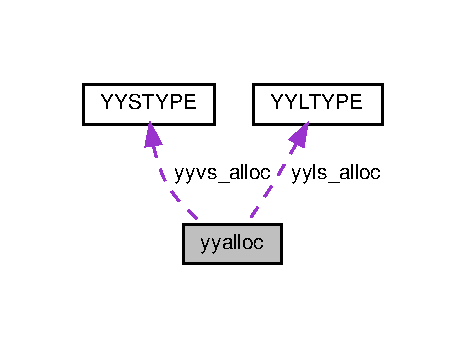
\includegraphics[width=224pt]{unionyyalloc__coll__graph}
\end{center}
\end{figure}
\subsection*{Public Attributes}
\begin{DoxyCompactItemize}
\item 
\mbox{\Hypertarget{unionyyalloc_a4800e0520a89a4789afa7b5d82197e65}\label{unionyyalloc_a4800e0520a89a4789afa7b5d82197e65}} 
yytype\+\_\+int16 {\bfseries yyss\+\_\+alloc}
\item 
\mbox{\Hypertarget{unionyyalloc_a9326f4fdc6f737a929444427836d8928}\label{unionyyalloc_a9326f4fdc6f737a929444427836d8928}} 
\hyperlink{unionYYSTYPE}{Y\+Y\+S\+T\+Y\+PE} {\bfseries yyvs\+\_\+alloc}
\item 
\mbox{\Hypertarget{unionyyalloc_a542e43248e6afac9af342c2f4e3162fc}\label{unionyyalloc_a542e43248e6afac9af342c2f4e3162fc}} 
\hyperlink{structYYLTYPE}{Y\+Y\+L\+T\+Y\+PE} {\bfseries yyls\+\_\+alloc}
\end{DoxyCompactItemize}


The documentation for this union was generated from the following file\+:\begin{DoxyCompactItemize}
\item 
parser.\+cpp\end{DoxyCompactItemize}

\hypertarget{structYYLTYPE}{}\section{Y\+Y\+L\+T\+Y\+PE Struct Reference}
\label{structYYLTYPE}\index{Y\+Y\+L\+T\+Y\+PE@{Y\+Y\+L\+T\+Y\+PE}}
\subsection*{Public Attributes}
\begin{DoxyCompactItemize}
\item 
\mbox{\Hypertarget{structYYLTYPE_a50ad3435eaea74bcab6f1ae5fbaefd89}\label{structYYLTYPE_a50ad3435eaea74bcab6f1ae5fbaefd89}} 
int {\bfseries first\+\_\+line}
\item 
\mbox{\Hypertarget{structYYLTYPE_a3a556533babab1b9066fa9bdbb809210}\label{structYYLTYPE_a3a556533babab1b9066fa9bdbb809210}} 
int {\bfseries first\+\_\+column}
\item 
\mbox{\Hypertarget{structYYLTYPE_a3075f2bc3448df5d2a9f16d22bff2cc1}\label{structYYLTYPE_a3075f2bc3448df5d2a9f16d22bff2cc1}} 
int {\bfseries last\+\_\+line}
\item 
\mbox{\Hypertarget{structYYLTYPE_acf87f8c98686f286eaf700c4b62157b2}\label{structYYLTYPE_acf87f8c98686f286eaf700c4b62157b2}} 
int {\bfseries last\+\_\+column}
\end{DoxyCompactItemize}


The documentation for this struct was generated from the following file\+:\begin{DoxyCompactItemize}
\item 
parser.\+h\end{DoxyCompactItemize}

\hypertarget{unionYYSTYPE}{}\section{Y\+Y\+S\+T\+Y\+PE Union Reference}
\label{unionYYSTYPE}\index{Y\+Y\+S\+T\+Y\+PE@{Y\+Y\+S\+T\+Y\+PE}}


{\ttfamily \#include $<$parser.\+h$>$}

\subsection*{Public Attributes}
\begin{DoxyCompactItemize}
\item 
char $\ast$ \hyperlink{unionYYSTYPE_a48739ab48c4c859d0411bdc538f46a4f}{S\+T\+R\+I\+NG}
\item 
\mbox{\Hypertarget{unionYYSTYPE_a61e375237e5938b15787439d72067515}\label{unionYYSTYPE_a61e375237e5938b15787439d72067515}} 
char $\ast$ {\bfseries N\+UM}
\end{DoxyCompactItemize}


\subsection{Detailed Description}
Value type. 

\subsection{Member Data Documentation}
\mbox{\Hypertarget{unionYYSTYPE_a48739ab48c4c859d0411bdc538f46a4f}\label{unionYYSTYPE_a48739ab48c4c859d0411bdc538f46a4f}} 
\index{Y\+Y\+S\+T\+Y\+PE@{Y\+Y\+S\+T\+Y\+PE}!S\+T\+R\+I\+NG@{S\+T\+R\+I\+NG}}
\index{S\+T\+R\+I\+NG@{S\+T\+R\+I\+NG}!Y\+Y\+S\+T\+Y\+PE@{Y\+Y\+S\+T\+Y\+PE}}
\subsubsection{\texorpdfstring{S\+T\+R\+I\+NG}{STRING}}
{\footnotesize\ttfamily char$\ast$ Y\+Y\+S\+T\+Y\+P\+E\+::\+S\+T\+R\+I\+NG}

yacc.\+c\+:1909 

The documentation for this union was generated from the following file\+:\begin{DoxyCompactItemize}
\item 
parser.\+h\end{DoxyCompactItemize}

%--- End generated contents ---

% Index
\backmatter
\newpage
\phantomsection
\clearemptydoublepage
\addcontentsline{toc}{chapter}{Index}
\printindex

\end{document}
